%% bare_jrnl.tex
%% V1.4b
%% 2015/08/26
%% by Michael Shell
%% see http://www.michaelshell.org/
%% for current contact information.
%%
%% This is a skeleton file demonstrating the use of IEEEtran.cls
%% (requires IEEEtran.cls version 1.8b or later) with an IEEE
%% journal paper.
%%
%% Support sites:
%% http://www.michaelshell.org/tex/ieeetran/
%% http://www.ctan.org/pkg/ieeetran
%% and
%% http://www.ieee.org/

%%*************************************************************************
%% Legal Notice:
%% This code is offered as-is without any warranty either expressed or
%% implied; without even the implied warranty of MERCHANTABILITY or
%% FITNESS FOR A PARTICULAR PURPOSE! 
%% User assumes all risk.
%% In no event shall the IEEE or any contributor to this code be liable for
%% any damages or losses, including, but not limited to, incidental,
%% consequential, or any other damages, resulting from the use or misuse
%% of any information contained here.
%%
%% All comments are the opinions of their respective authors and are not
%% necessarily endorsed by the IEEE.
%%
%% This work is distributed under the LaTeX Project Public License (LPPL)
%% ( http://www.latex-project.org/ ) version 1.3, and may be freely used,
%% distributed and modified. A copy of the LPPL, version 1.3, is included
%% in the base LaTeX documentation of all distributions of LaTeX released
%% 2003/12/01 or later.
%% Retain all contribution notices and credits.
%% ** Modified files should be clearly indicated as such, including  **
%% ** renaming them and changing author support contact information. **
%%*************************************************************************


% *** Authors should verify (and, if needed, correct) their LaTeX system  ***
% *** with the testflow diagnostic prior to trusting their LaTeX platform ***
% *** with production work. The IEEE's font choices and paper sizes can   ***
% *** trigger bugs that do not appear when using other class files.       ***                          ***
% The testflow support page is at:
% http://www.michaelshell.org/tex/testflow/

% If IEEEtran.cls has not been installed into the LaTeX system files,
% manually specify the path to it like:
\documentclass[journal]{IEEEtran}





% Some very useful LaTeX packages include:
% (uncomment the ones you want to load)


% *** MISC UTILITY PACKAGES ***
%
%\usepackage{ifpdf}
% Heiko Oberdiek's ifpdf.sty is very useful if you need conditional
% compilation based on whether the output is pdf or dvi.
% usage:
% \ifpdf
%   % pdf code
% \else
%   % dvi code
% \fi
% The latest version of ifpdf.sty can be obtained from:
% http://www.ctan.org/pkg/ifpdf
% Also, note that IEEEtran.cls V1.7 and later provides a builtin
% \ifCLASSINFOpdf conditional that works the same way.
% When switching from latex to pdflatex and vice-versa, the compiler may
% have to be run twice to clear warning/error messages.






% *** CITATION PACKAGES ***
%
\usepackage{cite}
% cite.sty was written by Donald Arseneau
% V1.6 and later of IEEEtran pre-defines the format of the cite.sty package
% \cite{} output to follow that of the IEEE. Loading the cite package will
% result in citation numbers being automatically sorted and properly
% "compressed/ranged". e.g., [1], [9], [2], [7], [5], [6] without using
% cite.sty will become [1], [2], [5]--[7], [9] using cite.sty. cite.sty's
% \cite will automatically add leading space, if needed. Use cite.sty's
% noadjust option (cite.sty V3.8 and later) if you want to turn this off
% such as if a citation ever needs to be enclosed in parenthesis.
% cite.sty is already installed on most LaTeX systems. Be sure and use
% version 5.0 (2009-03-20) and later if using hyperref.sty.
% The latest version can be obtained at:
% http://www.ctan.org/pkg/cite
% The documentation is contained in the cite.sty file itself.






% *** GRAPHICS RELATED PACKAGES ***
%

\ifCLASSINFOpdf
  \usepackage[pdftex]{graphicx}
  \graphicspath{ {./images/} }
  \DeclareGraphicsExtensions{.pdf,.jpeg,.png}
\else

  \usepackage[dvips]{graphicx}
  \graphicspath{{../eps/}}
  \DeclareGraphicsExtensions{.eps}
\fi
% graphicx was written by David Carlisle and Sebastian Rahtz. It is
% required if you want graphics, photos, etc. graphicx.sty is already
% installed on most LaTeX systems. The latest version and documentation
% can be obtained at: 
% http://www.ctan.org/pkg/graphicx
% Another good source of documentation is "Using Imported Graphics in
% LaTeX2e" by Keith Reckdahl which can be found at:
% http://www.ctan.org/pkg/epslatex
%
% latex, and pdflatex in dvi mode, support graphics in encapsulated
% postscript (.eps) format. pdflatex in pdf mode supports graphics
% in .pdf, .jpeg, .png and .mps (metapost) formats. Users should ensure
% that all non-photo figures use a vector format (.eps, .pdf, .mps) and
% not a bitmapped formats (.jpeg, .png). The IEEE frowns on bitmapped formats
% which can result in "jaggedy"/blurry rendering of lines and letters as
% well as large increases in file sizes.
%
% You can find documentation about the pdfTeX application at:
% http://www.tug.org/applications/pdftex




\usepackage{lscape}
\usepackage{rotating}
\usepackage{tikz}
% *** MATH PACKAGES ***
%
\usepackage{amsmath}
% A popular package from the American Mathematical Society that provides
% many useful and powerful commands for dealing with mathematics.
%
% Note that the amsmath package sets \interdisplaylinepenalty to 10000
% thus preventing page breaks from occurring within multiline equations. Use:
%\interdisplaylinepenalty=2500
% after loading amsmath to restore such page breaks as IEEEtran.cls normally
% does. amsmath.sty is already installed on most LaTeX systems. The latest
% version and documentation can be obtained at:
% http://www.ctan.org/pkg/amsmath





% *** SPECIALIZED LIST PACKAGES ***
%
\usepackage{algorithmic}
% algorithmic.sty was written by Peter Williams and Rogerio Brito.
% This package provides an algorithmic environment fo describing algorithms.
% You can use the algorithmic environment in-text or within a figure
% environment to provide for a floating algorithm. Do NOT use the algorithm
% floating environment provided by algorithm.sty (by the same authors) or
% algorithm2e.sty (by Christophe Fiorio) as the IEEE does not use dedicated
% algorithm float types and packages that provide these will not provide
% correct IEEE style captions. The latest version and documentation of
% algorithmic.sty can be obtained at:
% http://www.ctan.org/pkg/algorithms
% Also of interest may be the (relatively newer and more customizable)
% algorithmicx.sty package by Szasz Janos:
% http://www.ctan.org/pkg/algorithmicx




% *** ALIGNMENT PACKAGES ***
%
\usepackage{array}
% Frank Mittelbach's and David Carlisle's array.sty patches and improves
% the standard LaTeX2e array and tabular environments to provide better
% appearance and additional user controls. As the default LaTeX2e table
% generation code is lacking to the point of almost being broken with
% respect to the quality of the end results, all users are strongly
% advised to use an enhanced (at the very least that provided by array.sty)
% set of table tools. array.sty is already installed on most systems. The
% latest version and documentation can be obtained at:
% http://www.ctan.org/pkg/array


% IEEEtran contains the IEEEeqnarray family of commands that can be used to
% generate multiline equations as well as matrices, tables, etc., of high
% quality.




% *** SUBFIGURE PACKAGES ***
\ifCLASSOPTIONcompsoc
  \usepackage[caption=false,font=normalsize,labelfont=sf,textfont=sf]{subfig}
\else
  \usepackage[caption=false,font=footnotesize]{subfig}
\fi
% subfig.sty, written by Steven Douglas Cochran, is the modern replacement
% for subfigure.sty, the latter of which is no longer maintained and is
% incompatible with some LaTeX packages including fixltx2e. However,
% subfig.sty requires and automatically loads Axel Sommerfeldt's caption.sty
% which will override IEEEtran.cls' handling of captions and this will result
% in non-IEEE style figure/table captions. To prevent this problem, be sure
% and invoke subfig.sty's "caption=false" package option (available since
% subfig.sty version 1.3, 2005/06/28) as this is will preserve IEEEtran.cls
% handling of captions.
% Note that the Computer Society format requires a larger sans serif font
% than the serif footnote size font used in traditional IEEE formatting
% and thus the need to invoke different subfig.sty package options depending
% on whether compsoc mode has been enabled.
%
% The latest version and documentation of subfig.sty can be obtained at:
% http://www.ctan.org/pkg/subfig




% *** FLOAT PACKAGES ***
%
\usepackage{fixltx2e}
% fixltx2e, the successor to the earlier fix2col.sty, was written by
% Frank Mittelbach and David Carlisle. This package corrects a few problems
% in the LaTeX2e kernel, the most notable of which is that in current
% LaTeX2e releases, the ordering of single and double column floats is not
% guaranteed to be preserved. Thus, an unpatched LaTeX2e can allow a
% single column figure to be placed prior to an earlier double column
% figure.
% Be aware that LaTeX2e kernels dated 2015 and later have fixltx2e.sty's
% corrections already built into the system in which case a warning will
% be issued if an attempt is made to load fixltx2e.sty as it is no longer
% needed.
% The latest version and documentation can be found at:
% http://www.ctan.org/pkg/fixltx2e


%\usepackage{stfloats}
% stfloats.sty was written by Sigitas Tolusis. This package gives LaTeX2e
% the ability to do double column floats at the bottom of the page as well
% as the top. (e.g., "\begin{figure*}[!b]" is not normally possible in
% LaTeX2e). It also provides a command:
%\fnbelowfloat
% to enable the placement of footnotes below bottom floats (the standard
% LaTeX2e kernel puts them above bottom floats). This is an invasive package
% which rewrites many portions of the LaTeX2e float routines. It may not work
% with other packages that modify the LaTeX2e float routines. The latest
% version and documentation can be obtained at:
% http://www.ctan.org/pkg/stfloats
% Do not use the stfloats baselinefloat ability as the IEEE does not allow
% \baselineskip to stretch. Authors submitting work to the IEEE should note
% that the IEEE rarely uses double column equations and that authors should try
% to avoid such use. Do not be tempted to use the cuted.sty or midfloat.sty
% packages (also by Sigitas Tolusis) as the IEEE does not format its papers in
% such ways.
% Do not attempt to use stfloats with fixltx2e as they are incompatible.
% Instead, use Morten Hogholm'a dblfloatfix which combines the features
% of both fixltx2e and stfloats:
%
% \usepackage{dblfloatfix}
% The latest version can be found at:
% http://www.ctan.org/pkg/dblfloatfix




%\ifCLASSOPTIONcaptionsoff
%  \usepackage[nomarkers]{endfloat}
% \let\MYoriglatexcaption\caption
% \renewcommand{\caption}[2][\relax]{\MYoriglatexcaption[#2]{#2}}
%\fi
% endfloat.sty was written by James Darrell McCauley, Jeff Goldberg and 
% Axel Sommerfeldt. This package may be useful when used in conjunction with 
% IEEEtran.cls'  captionsoff option. Some IEEE journals/societies require that
% submissions have lists of figures/tables at the end of the paper and that
% figures/tables without any captions are placed on a page by themselves at
% the end of the document. If needed, the draftcls IEEEtran class option or
% \CLASSINPUTbaselinestretch interface can be used to increase the line
% spacing as well. Be sure and use the nomarkers option of endfloat to
% prevent endfloat from "marking" where the figures would have been placed
% in the text. The two hack lines of code above are a slight modification of
% that suggested by in the endfloat docs (section 8.4.1) to ensure that
% the full captions always appear in the list of figures/tables - even if
% the user used the short optional argument of \caption[]{}.
% IEEE papers do not typically make use of \caption[]'s optional argument,
% so this should not be an issue. A similar trick can be used to disable
% captions of packages such as subfig.sty that lack options to turn off
% the subcaptions:
% For subfig.sty:
% \let\MYorigsubfloat\subfloat
% \renewcommand{\subfloat}[2][\relax]{\MYorigsubfloat[]{#2}}
% However, the above trick will not work if both optional arguments of
% the \subfloat command are used. Furthermore, there needs to be a
% description of each subfigure *somewhere* and endfloat does not add
% subfigure captions to its list of figures. Thus, the best approach is to
% avoid the use of subfigure captions (many IEEE journals avoid them anyway)
% and instead reference/explain all the subfigures within the main caption.
% The latest version of endfloat.sty and its documentation can obtained at:
% http://www.ctan.org/pkg/endfloat
%
% The IEEEtran \ifCLASSOPTIONcaptionsoff conditional can also be used
% later in the document, say, to conditionally put the References on a 
% page by themselves.




% *** PDF, URL AND HYPERLINK PACKAGES ***
%
\usepackage{url}
% url.sty was written by Donald Arseneau. It provides better support for
% handling and breaking URLs. url.sty is already installed on most LaTeX
% systems. The latest version and documentation can be obtained at:
% http://www.ctan.org/pkg/url
% Basically, \url{my_url_here}.




% *** Do not adjust lengths that control margins, column widths, etc. ***
% *** Do not use packages that alter fonts (such as pslatex).         ***
% There should be no need to do such things with IEEEtran.cls V1.6 and later.
% (Unless specifically asked to do so by the journal or conference you plan
% to submit to, of course. )


% correct bad hyphenation here
\hyphenation{op-tical net-works semi-conduc-tor}


\begin{document}

%
% paper title
% Titles are generally capitalized except for words such as a, an, and, as,
% at, but, by, for, in, nor, of, on, or, the, to and up, which are usually
% not capitalized unless they are the first or last word of the title.
% Linebreaks \\ can be used within to get better formatting as desired.
% Do not put math or special symbols in the title.
\title{CE888 Assignment 2}
%
%
% author names and IEEE memberships
% note positions of commas and nonbreaking spaces ( ~ ) LaTeX will not break
% a structure at a ~ so this keeps an author's name from being broken across
% two lines.
% use \thanks{} to gain access to the first footnote area
% a separate \thanks must be used for each paragraph as LaTeX2e's \thanks
% was not built to handle multiple paragraphs
%

\author{Ogulcan~Ozer}% <-this % stops a space


% note the % following the last \IEEEmembership and also \thanks - 
% these prevent an unwanted space from occurring between the last author name
% and the end of the author line. i.e., if you had this:
% 
% \author{....lastname \thanks{...} \thanks{...} }
%                     ^------------^------------^----Do not want these spaces!
%
% a space would be appended to the last name and could cause every name on that
% line to be shifted left slightly. This is one of those "LaTeX things". For
% instance, "\textbf{A} \textbf{B}" will typeset as "A B" not "AB". To get
% "AB" then you have to do: "\textbf{A}\textbf{B}"
% \thanks is no different in this regard, so shield the last } of each \thanks
% that ends a line with a % and do not let a space in before the next \thanks.
% Spaces after \IEEEmembership other than the last one are OK (and needed) as
% you are supposed to have spaces between the names. For what it is worth,
% this is a minor point as most people would not even notice if the said evil
% space somehow managed to creep in.



% The paper headers
\markboth{University of Essex School of Computer Science and Electronic Engineering}%
{University of Essex School of Computer Science and Electronic Engineering}
% The only time the second header will appear is for the odd numbered pages
% after the title page when using the twoside option.
% 
% *** Note that you probably will NOT want to include the author's ***
% *** name in the headers of peer review papers.                   ***
% You can use \ifCLASSOPTIONpeerreview for conditional compilation here if
% you desire.




% If you want to put a publisher's ID mark on the page you can do it like
% this:
%\IEEEpubid{0000--0000/00\$00.00~\copyright~2015 IEEE}
% Remember, if you use this you must call \IEEEpubidadjcol in the second
% column for its text to clear the IEEEpubid mark.



% use for special paper notices
%\IEEEspecialpapernotice{(Invited Paper)}




% make the title area
\maketitle

% As a general rule, do not put math, special symbols or citations
% in the abstract or keywords.
\begin{abstract}
In this work, we explore autoencoders with a hidden softmax layer as a clustering method, by training an autoencoder and using the maximum of the output vector as our cluster assignment. 
We also examine traditioanl clustering algorithms and experiment with feature selection methods to see how they perform compared to each other. 
\end{abstract}


% For peer review papers, you can put extra information on the cover
% page as needed:
% \ifCLASSOPTIONpeerreview
% \begin{center} \bfseries EDICS Category: 3-BBND \end{center}
% \fi
%
% For peerreview papers, this IEEEtran command inserts a page break and
% creates the second title. It will be ignored for other modes.
\IEEEpeerreviewmaketitle



\section{Introduction}
% The very first letter is a 2 line initial drop letter followed
% by the rest of the first word in caps.
% 
% form to use if the first word consists of a single letter:
% \IEEEPARstart{A}{demo} file is ....
% 
% form to use if you need the single drop letter followed by
% normal text (unknown if ever used by the IEEE):
% \IEEEPARstart{A}{}demo file is ....
% 
% Some journals put the first two words in caps:
% \IEEEPARstart{T}{his demo} file is ....
% 
% Here we have the typical use of a "T" for an initial drop letter
% and "HIS" in caps to complete the first word.
\IEEEPARstart{U}{nsupervised} learning is a branch of machine learning that deals with unlabeled data to find patterns, groups
and relations. This sub section of machine learning is useful to describe and understand unknown data, which 
also helps us understand the properties of future data samples. Right now we are collecting data much faster than we can process it.
And most of the time the data we acquire is unlabeled, and these huge amounts of data are complex, noisy
and it might include unnecessary information.\par There are different ways to reduce the complexity of a given data and learn good 
features from it. In this work, we looked at PCA and autoencoders. 
Autoencoders are a part of representational learning, which can be trained with or without labels.
They play a key role in deep learning applications. They are used in dimensionality reduction and feature 
extraction, and together with deep learning they gained a lot of traction after Hinton proposed a method to train 
deep belief networks one layer at a time \cite{hinton2006fast}. Another addition to the autoencoders and PCA was assigning the data to clusters usnig the softmax activation function.
Since softmax gives us the probability distribution over-the classes of our data- the output vector \cite[pp. 178-181]{goodfellow2016deep}, we can use the output of our
encoder for cluster assignment. The motivation for using autoencoders is, in what they do they are
very similar to traditional feature selection algorithms, but they are also capable of learning good features from
complex and high dimensional data. This aspect of autoencoders and unsupervised learning in general is important. 
As LeCun states in \cite{lecun2015deep}, people are not paying attention to unsupervised learning because of the success of the supervised learning
in recent years. But it will be far more important in the future because of how living beings perceive and learn, they do not
need labels to recognize the world around them.\par In this paper  In Section III, We explain the tools we used and mentioned the implementation steps we took for the experiments. Then we present the datasets that we used for the task and give detailed information about them.The detailed experiments and analyses for the task will be mentioned in Section IV.
Finally, we talk about how we evaluated our models and we discuss the results.

\section{Background}
Clustering is used to naturally group the samples in order to extract information or make decisions\cite{jain1999data}.
Autoencoders were discovered in 1985 and presented in\cite{rumelhart1985learning}. As the technology and our computational power improved immensely in the last decade, they became more and more feasible. After Hinton's solution\cite{hinton2006fast} these simple network models became very popular, now they are used in the state-of-the-art machine learning models, breaking records and in some tasks performing better than humans\cite{schmidhuber2015deep}. But most of the success and interest to the autoencoders can be attributed to the studies on supervised learning.\par
In this study, first we looked at the well-known traditional models k-Means\cite{macqueen1967some} and DBSCAN\cite{ester1996density}. K-Means tries to divide the data into k clusters which are defined by k centroids. Each sample given to the algorithm is assigned to the cluster with the nearest mean. The k-Means algorithm is not deterministic and results in different clusters for different initializations. DBSCAN on the other hand separates the data by looking at it as highly populated areas that are separated by low population areas. The DBSCAN algorithm, as opposed to k-Means, is deterministic and results in same clusters.

After the traditional methods, we trained different autoencoders for dimensionality reduction and clustering. The model of our autoencoder networks is a simple end to end auto encoder with one hidden layer.
\begin{figure}[!ht]
  \centering
  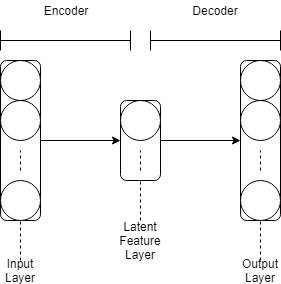
\includegraphics[width=2.5in]{images/ae_model.png}
  \caption{Autoencoder model
  }
  \label{fig_ae_model}
  \end{figure}
First model uses linear activation functions, in order to achieve PCA-like behavior. Then our second autoencoder model uses non-linear sigmoid activation function, for the purpose of learning good features from high-dimensional data. 
\begin{equation}
  \sigma(a)=\frac{1}{1+e^{-a}}
\end{equation}
The output of these two models are used as the inputs to the traditional clustering algorithms. 
Finally, our last model uses a softmax activation function in the latent feature layer. Softmax provides the probability distribution over the nodes of our latent feature layer. Which are then used to cluster the data
\begin{equation}
  softmax_i(a)=\frac{\exp{a_i}}{\sum\exp{a_i}}
\end{equation}


Even though the k-Means algorithm cannot cluster non-linear data, \cite{xie2016unsupervised} and \cite{salakhutdinov2007learning} show that traditional clustering methods can be improved significantly if a good feature selection method is applied before the clustering procedure. In \cite{hinton2006reducing} feature selection with autoencoders are compared to other feature selection methods like PCA , non-linear PCA etc. And it is stated that the autoencoders perform better than these techniques if they are initialized and trained carefully. Another study\cite{poultney2007efficient} learns overcomplete representations of features for data reconstructions. It is shown in their results that this sparse, energy based autoencoder with linear layers can reproduce the MINST dataset with 0.7\% error, while not requiring any preprocessing.\cite{le2011building} also follows a similar approach, in which a deep sparse network trained in unsupervised fashion to recognize faces, humans and objects..
  \par
The most similar work \cite{xie2016unsupervised} uses stacked denoising autoencoders to extract good features for clustering. When the pre-training of their SAE is over, the trained encoder model is extracted and merged with a custom layer which applies softmax activation to the resulting output vector from the encoder. After setting up the final model, they use k-Means to generate cluster centroids for the data. Then, these centroids are used to train/fine-tune the final model by minimizing the KL-divergence between the soft assignment of the network and the cluster centroids created by k-Means. 


\section{Methodology}
In this study, we experimented with autoencoders using a softmax latent feature layer, to bin the data into the softmax nodes and use the maximum of this vector for our clustering assignment. But before testing our main objective, we first set up a base line specific for our datasets using the traditional clustering algorithms. We also looked into how feature selection procedures affect the performance of these clustering algorithms. First with PCA, then with linear autoencoders and finally with non-linear autoencoders. After creating the baseline and experimenting with feature selection, we proceeded to our main objective.
\par
Implementation of the tasks were done using Python. Reading the data files and importing procedures were implemented using the Pandas library. The traditional clustering algorithms were implemented using the scikit-learn library which already includes the k-Means and DBSCAN algorithms. Also some data processing operations like normalization/scaling, train-test split were done using the functions provided by scikit-learn. For the tasks related to autoencoders, TensorFlow and Keras libraries were used. Then, a high level autoencoder class was implemented in order to easily create autoencoders with desired layers, nodes and activation functions. Finally, the data presentation and plotting the results were done using matplotlib and seaborn libraries.
\par

The three datasets chosen to be clustered in this study are Modified NIST, Human Activity Recognition Using Smartphones (HAR) 
and High Time Resolution Universe Survey 2 (HTRU2).\par

MNIST is a image dataset of hand written digits. It is a modified version of the NIST dataset collected from Census Bureau employees and high-school
students and processed by LeCun et.al..The original NIST set was normalized, so that each sample would be centered
according to the weights of it's pixels in a 28x28 box. Images were also converted to grey-scale and shuffled to make it
easy to use in machine learning applications \cite{lecun1998gradient}. The dataset consists of 60.000 training images and 10.000 test images. Since each
sample is represented as a 28x28 pixel binary image, it can be said that samples have 784 features. MNIST dataset is frequently
used in machine learning research, which makes it easier for researchers to compare their models and solutions to the others
in the field.

\begin{figure}[!ht]
\centering
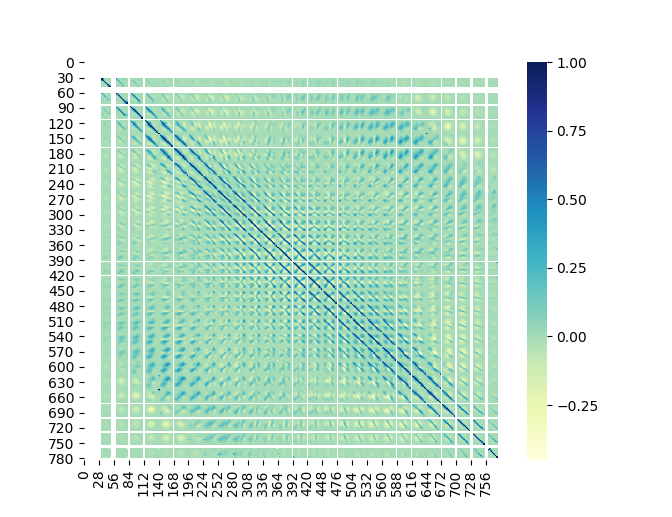
\includegraphics[width=2.5in]{images/cor_heat_mnist.png}
\caption{Corraletion heatmap of MNIST features.}
\label{fig_mnist}
\end{figure}

HAR is a dataset of multiple classes of human activities. It was created by recording different classes of activities of 30 volunteers
by using the accelerometer and the gyroscope in a smartphone. These sensors were used to record the linear acceleration and angular velocity
on three axes at 50 Hz. Volunteers were also recorded by a camera for the labeling of the activities (walking, walking upstairs, walking downstairs, sitting, standing, laying)\cite{anguita2013public}. The dataset consists of 7352
training samples and 2947 test samples. Each sample has 561 features which are- extracted- estimated from the recorded accelerometer and gyroscope signals. These features are normalized, scaled and shifted to be within [-1,1].  Subject id labels for the features and mentioned raw accelerometer and gyroscope signals are also provided with the dataset.
Dimensions of the subject ids are the same with their training and testing parts. On the other hand, the raw signals are separated into nine different files grouped under three axes, which are body acceleration (X,Y,Z), body gyroscope (X,Y,Z) and total acceleration (X,Y,Z).

\begin{figure}[!ht]
  \centering
  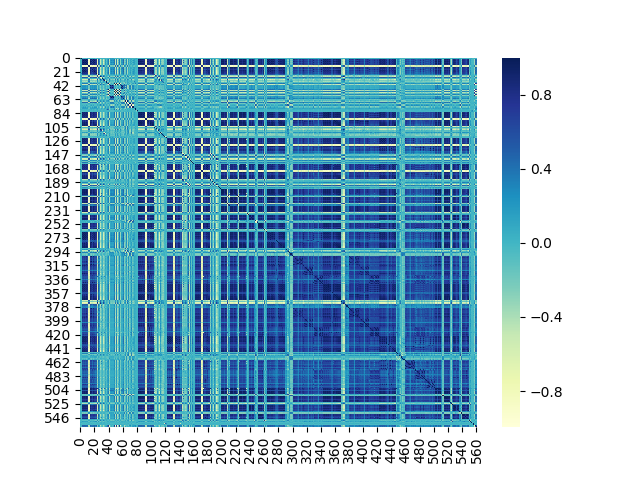
\includegraphics[width=2.5in]{images/cor_heat_har.png}
  \caption{Corraletion heatmap of HAR features.}
  \label{fig_har}
  \end{figure}
  \par
  
  Our last dataset HTRU2 was obtained by Bates\cite{bates2012high} using ANNs to first filter out the bad candidates, then manually inspecting the outputs of the ANN. Each sample of HTRU2 is a set of features extracted from the data acquired by large radio telescopes during High Time Resolution Universe Survey. HTRU2 has 8 features and consists of 17,898 total samples. Only 1,639 of them are positive pulsar samples and the 16,259 of them are negative samples. The first four features are simple statistics of the pulsar profiles and rest of the features were obtained from DM-SNR curve\cite{keith2010high}.These compact features were obtained from 90.000 labeled pulsar candidates by using Pulsar Feature Lab \cite{Lyon2015}.

  \begin{figure}[!ht]
    \centering
    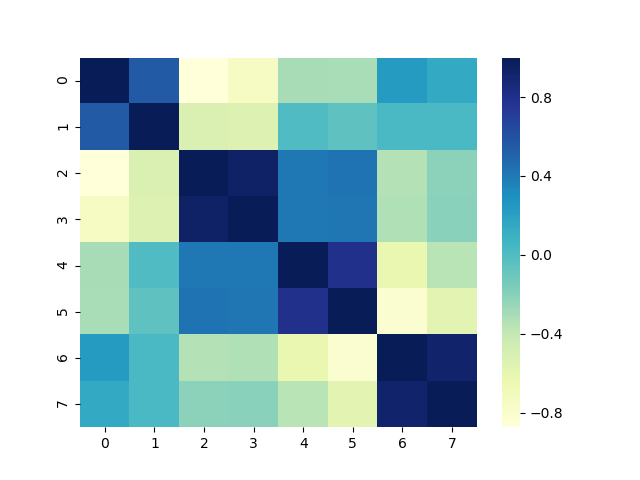
\includegraphics[width=2.5in]{images/cor_heat_htru.png}
    \caption{Corraletion heatmap of htru features.}
    \label{fig_htru}
    \end{figure}
    \par
  
  \begin{table}[!ht]
  %% increase table row spacing, adjust to taste
  \renewcommand{\arraystretch}{1.3}
  % if using array.sty, it might be a good idea to tweak the value of
  % \extrarowheight as needed to properly center the text within the cells
  \caption{Dataset statistics.}
  \label{tab_datasets}
  \centering
  %% Some packages, such as MDW tools, offer better commands for making tables
  %% than the plain LaTeX2e tabular which is used here.
  \begin{tabular}{|c||c|c|c|}
  \hline
  Datasets &    Data Points &  Features &  Classes \\
  \hline
  \hline
  MNIST &    70.000 &   784 &                 10 \\
  \hline
  HAR &       10.299 &   561 &                 6 \\
  \hline
  HTRU2 &    17,898 &   8 &                  2 \\
  \hline
  \end{tabular}
  \end{table}
\section{Experiments}
The experiments done in this work can be separated into three sub-groups. First part is the clustering algorithms. The second part is the effect of feature selection methods. And the third part is the clustering using the maximum of the softmax output vector. Before running the experiments, for repeatability purposes, the randomness states were fixed.  

\subsection{Clustering }

First, to have a base-line to compare our results we clustered our data using the k-Means algorithm. Since our datasets are labeled, we set the number of centroids k to the number of classes for each dataset, and we set the number of initializations to 10.

\begin{figure}[!ht]
  \centering
  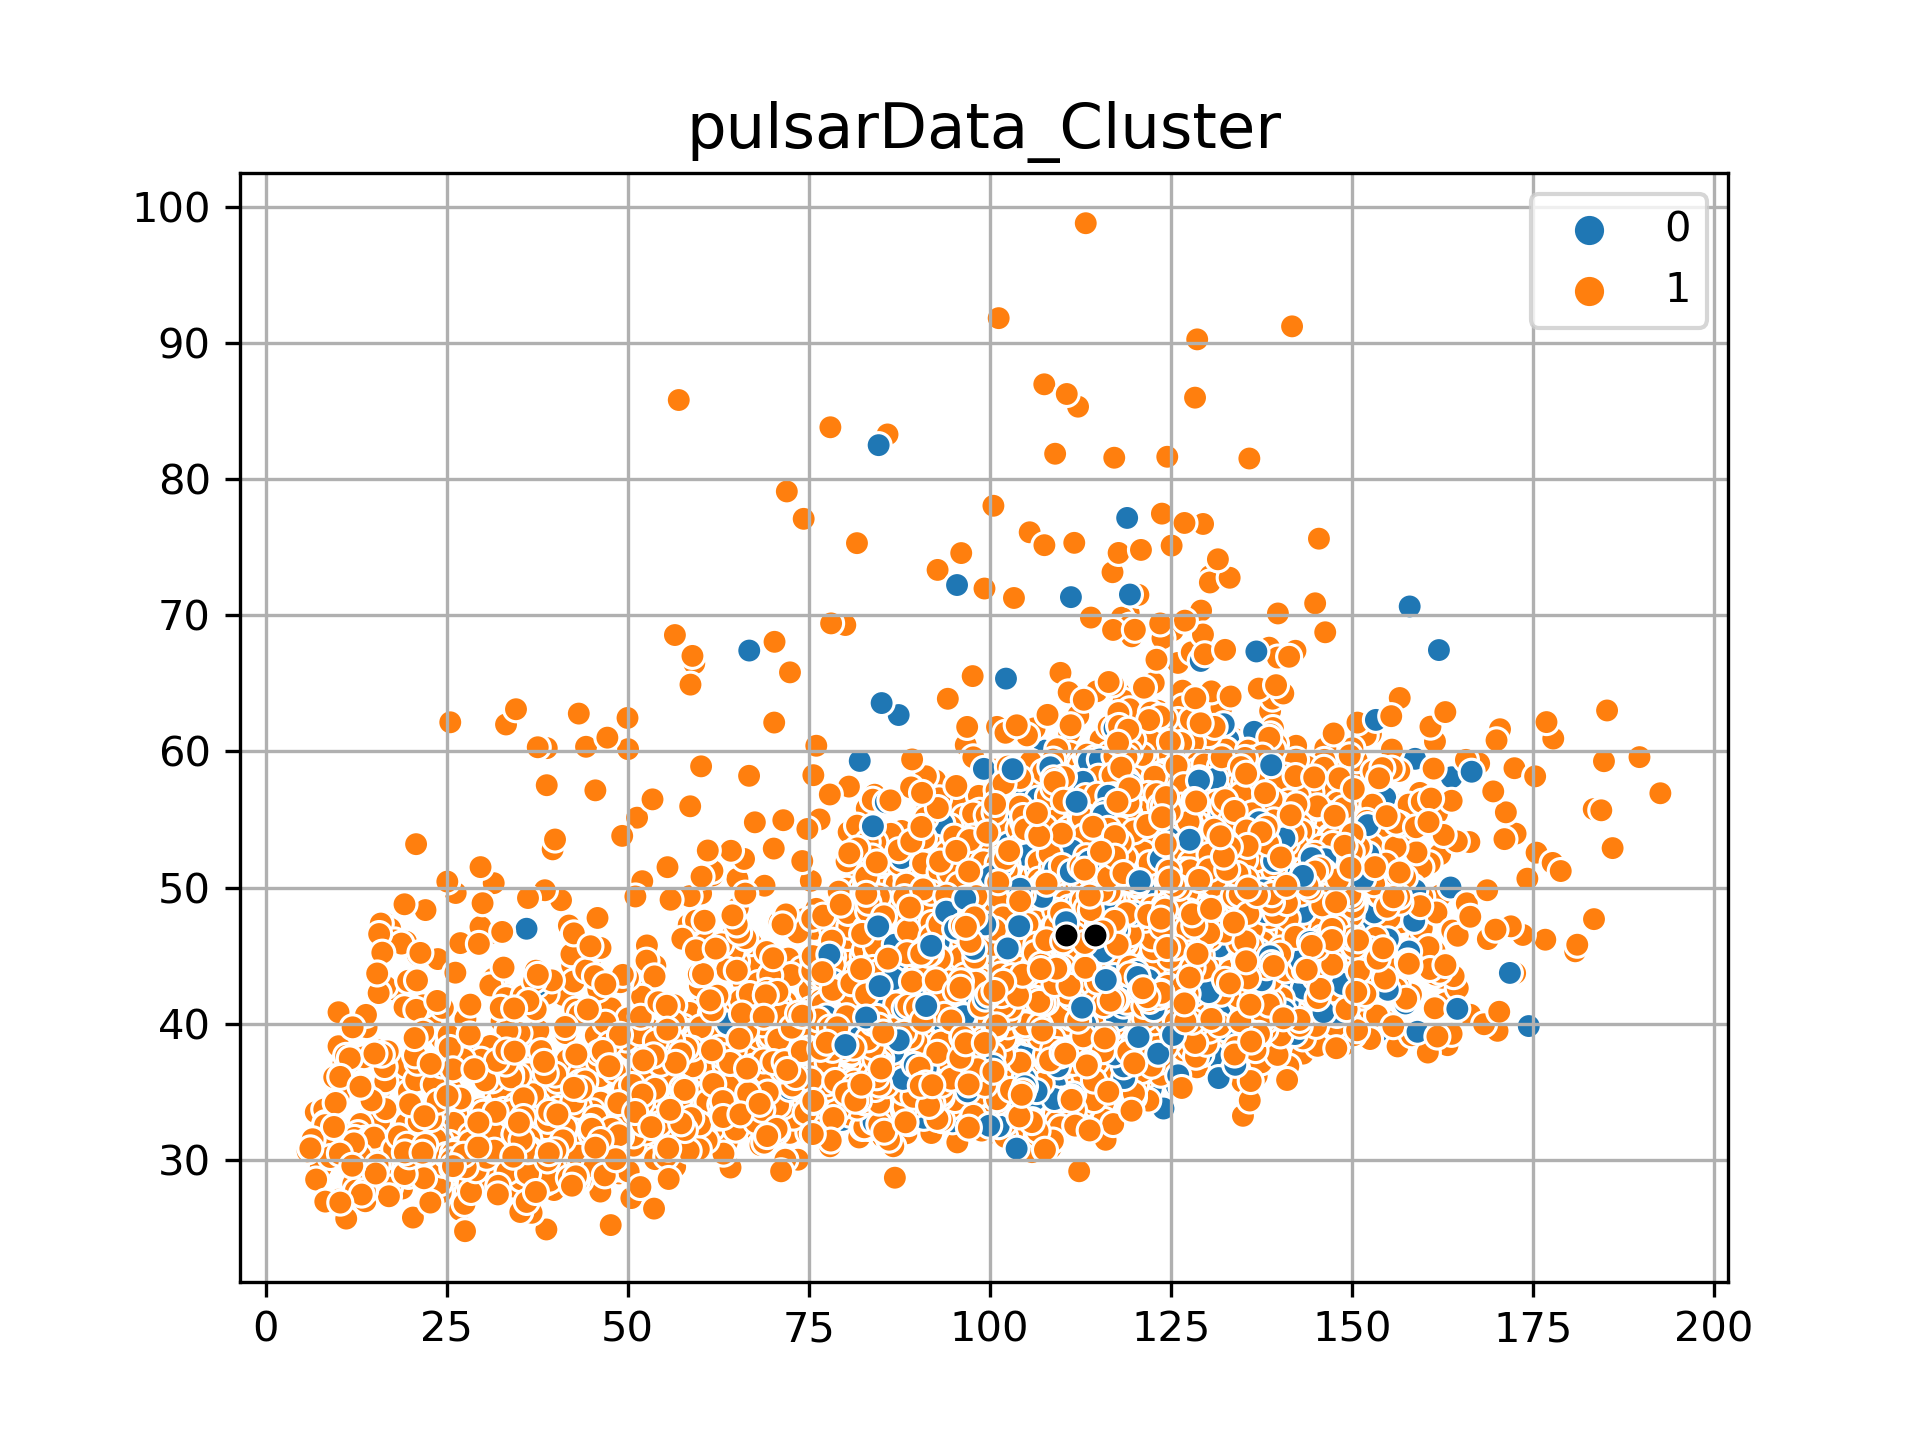
\includegraphics[width=3.3in]{images/pulsarData_Cluster.png}
  \caption{Plot of first two features of the HTRU dataset, clustered and labeled by k-Means}
  \label{fig_pulsarData_Cluster}
\end{figure}
\par

\begin{table}[!ht]
%% increase table row spacing, adjust to taste
\renewcommand{\arraystretch}{1.3}
% if using array.sty, it might be a good idea to tweak the value of
% \extrarowheight as needed to properly center the text within the cells
\caption{K-Means Clustering Results.}
\label{tab_kmeans_res}
\centering
\begin{tabular}{|c|c|c|c|c|}
\hline
Data - Method &  Homogenity &  Complete. &  V-Measure &  Accuracy \\
\hline
\hline
htru k-Means &    0.031206 &      0.023027 &   0.026500 &  0.234949 \\
\hline
har k-Means&    0.570123 &      0.600019 &   0.584689 &  0.289853 \\
\hline 
mnist k-Means&    0.486553 &      0.497699 &   0.492063 &  0.083400 \\
\hline
\end{tabular}
\end{table}


\begin{figure}[!ht]
  \centering
  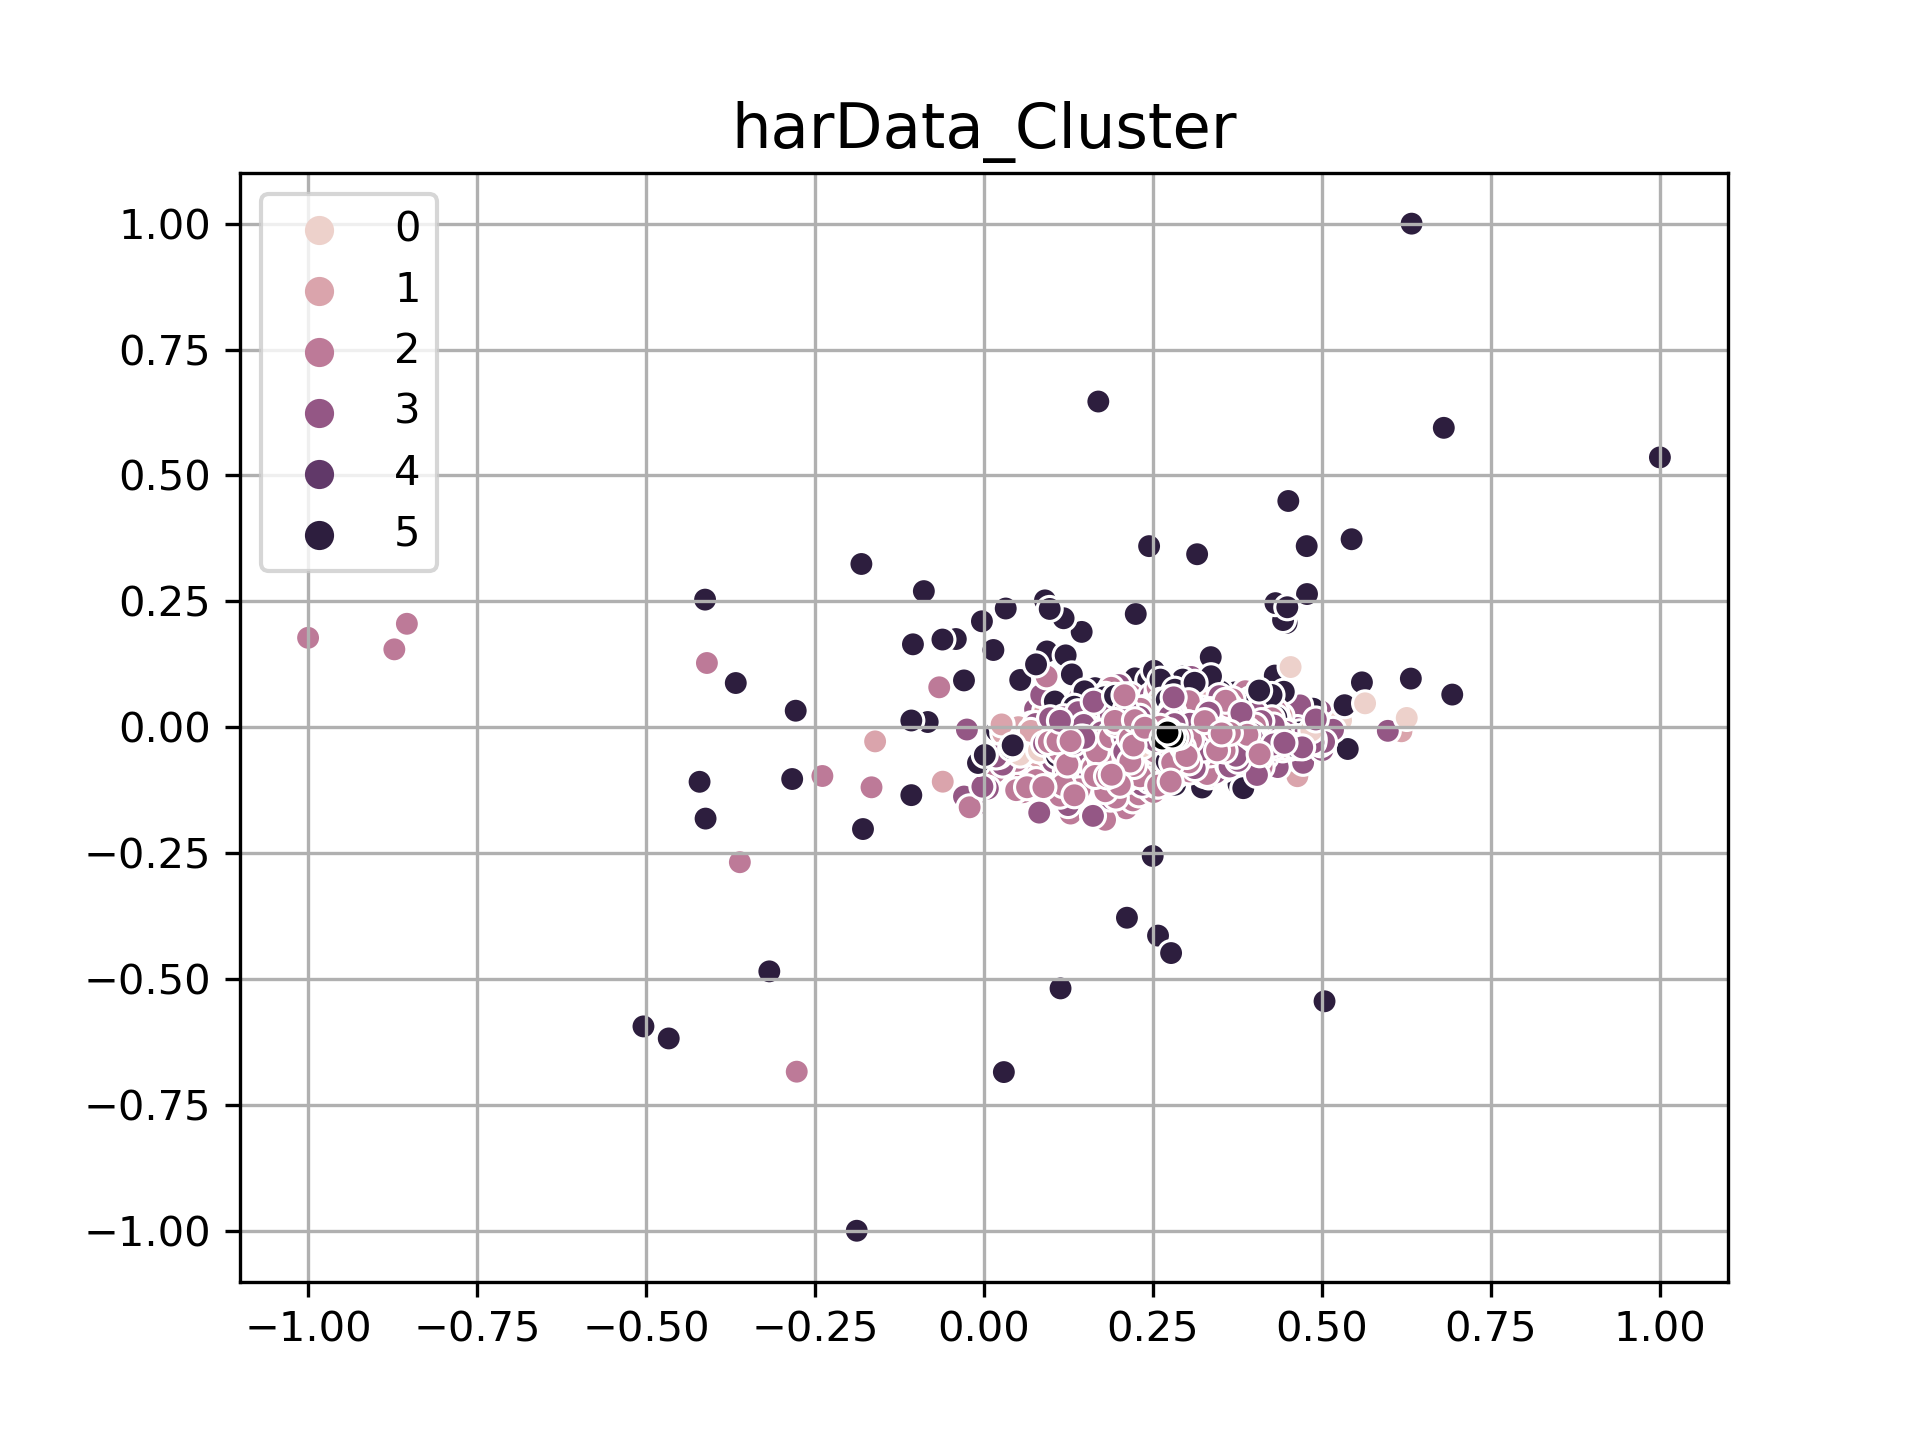
\includegraphics[width=3.3in]{images/harData_Cluster.png}
  \caption{Plot of first two features of the HAR dataset, clustered and labeled by k-Means}
  \label{fig_harData_Cluster}
\end{figure}
\par

In addition to the k-Means, DBSCAN algorithm was also used to cluster our datasets. But the DBSCAN algorithm provided by the scikit-learn library labeled our datasets as noise and failed to cluster them. Which we think is because of the high dimensionality of our data. Thus, the results of the DBSCAN algorithm were discarded. Also because of the poor results of the MNIST, all the centroids were stacked at the origin and its k-Means plot was not included here.

\begin{figure*}[!htb]
  \minipage{0.32\textwidth}
    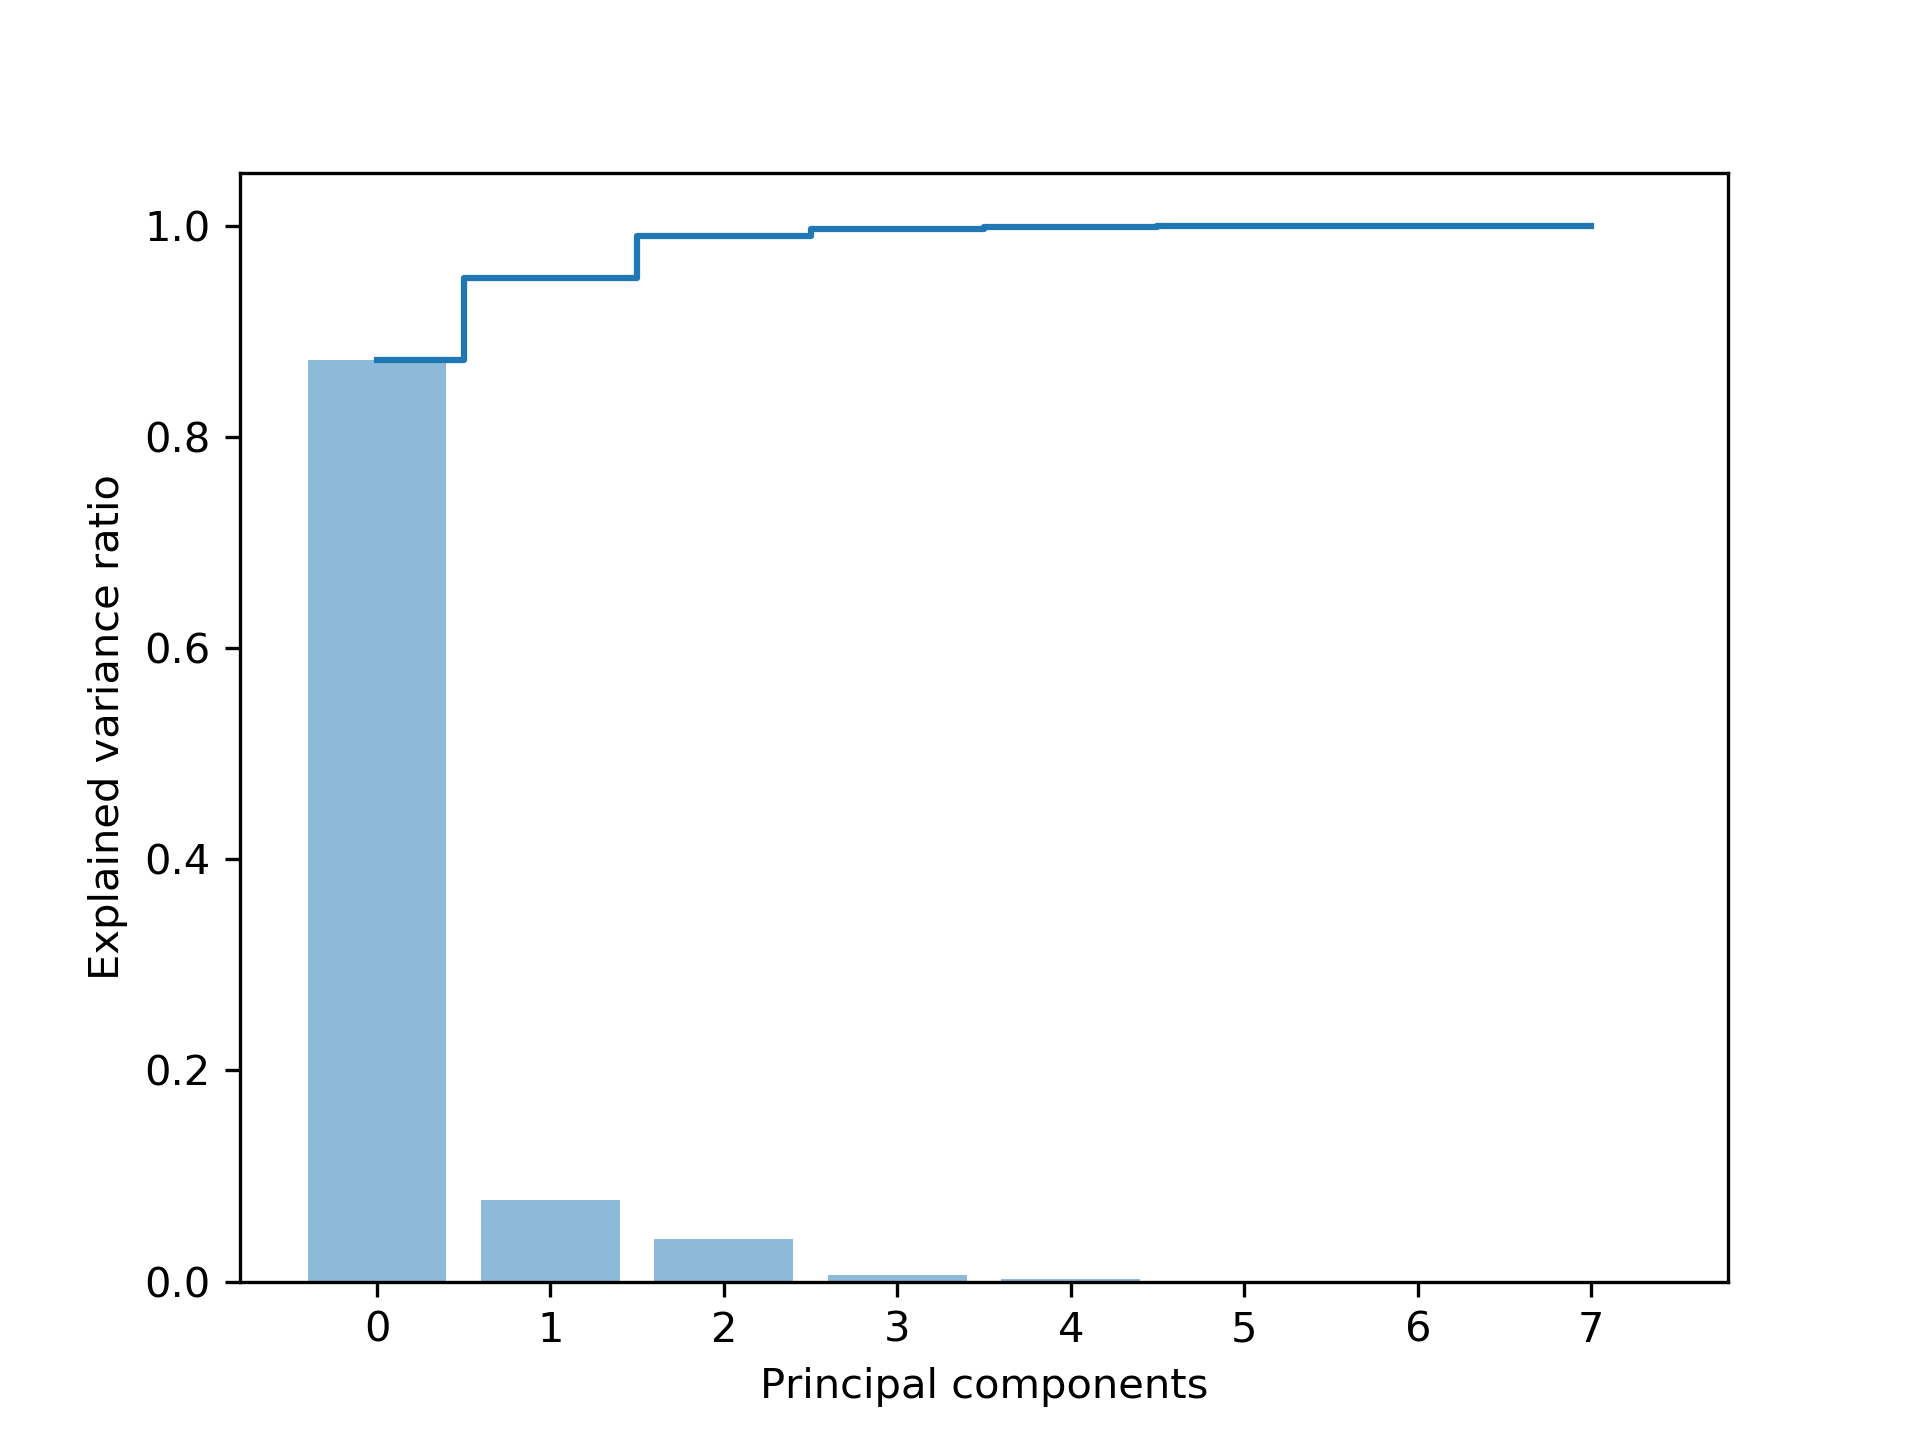
\includegraphics[width=\linewidth]{images/pulsarpca.png}
    \caption{HTRU Explained variance ratio.}\label{fig_pulsarpca}
  \endminipage\hfill
  \minipage{0.32\textwidth}
    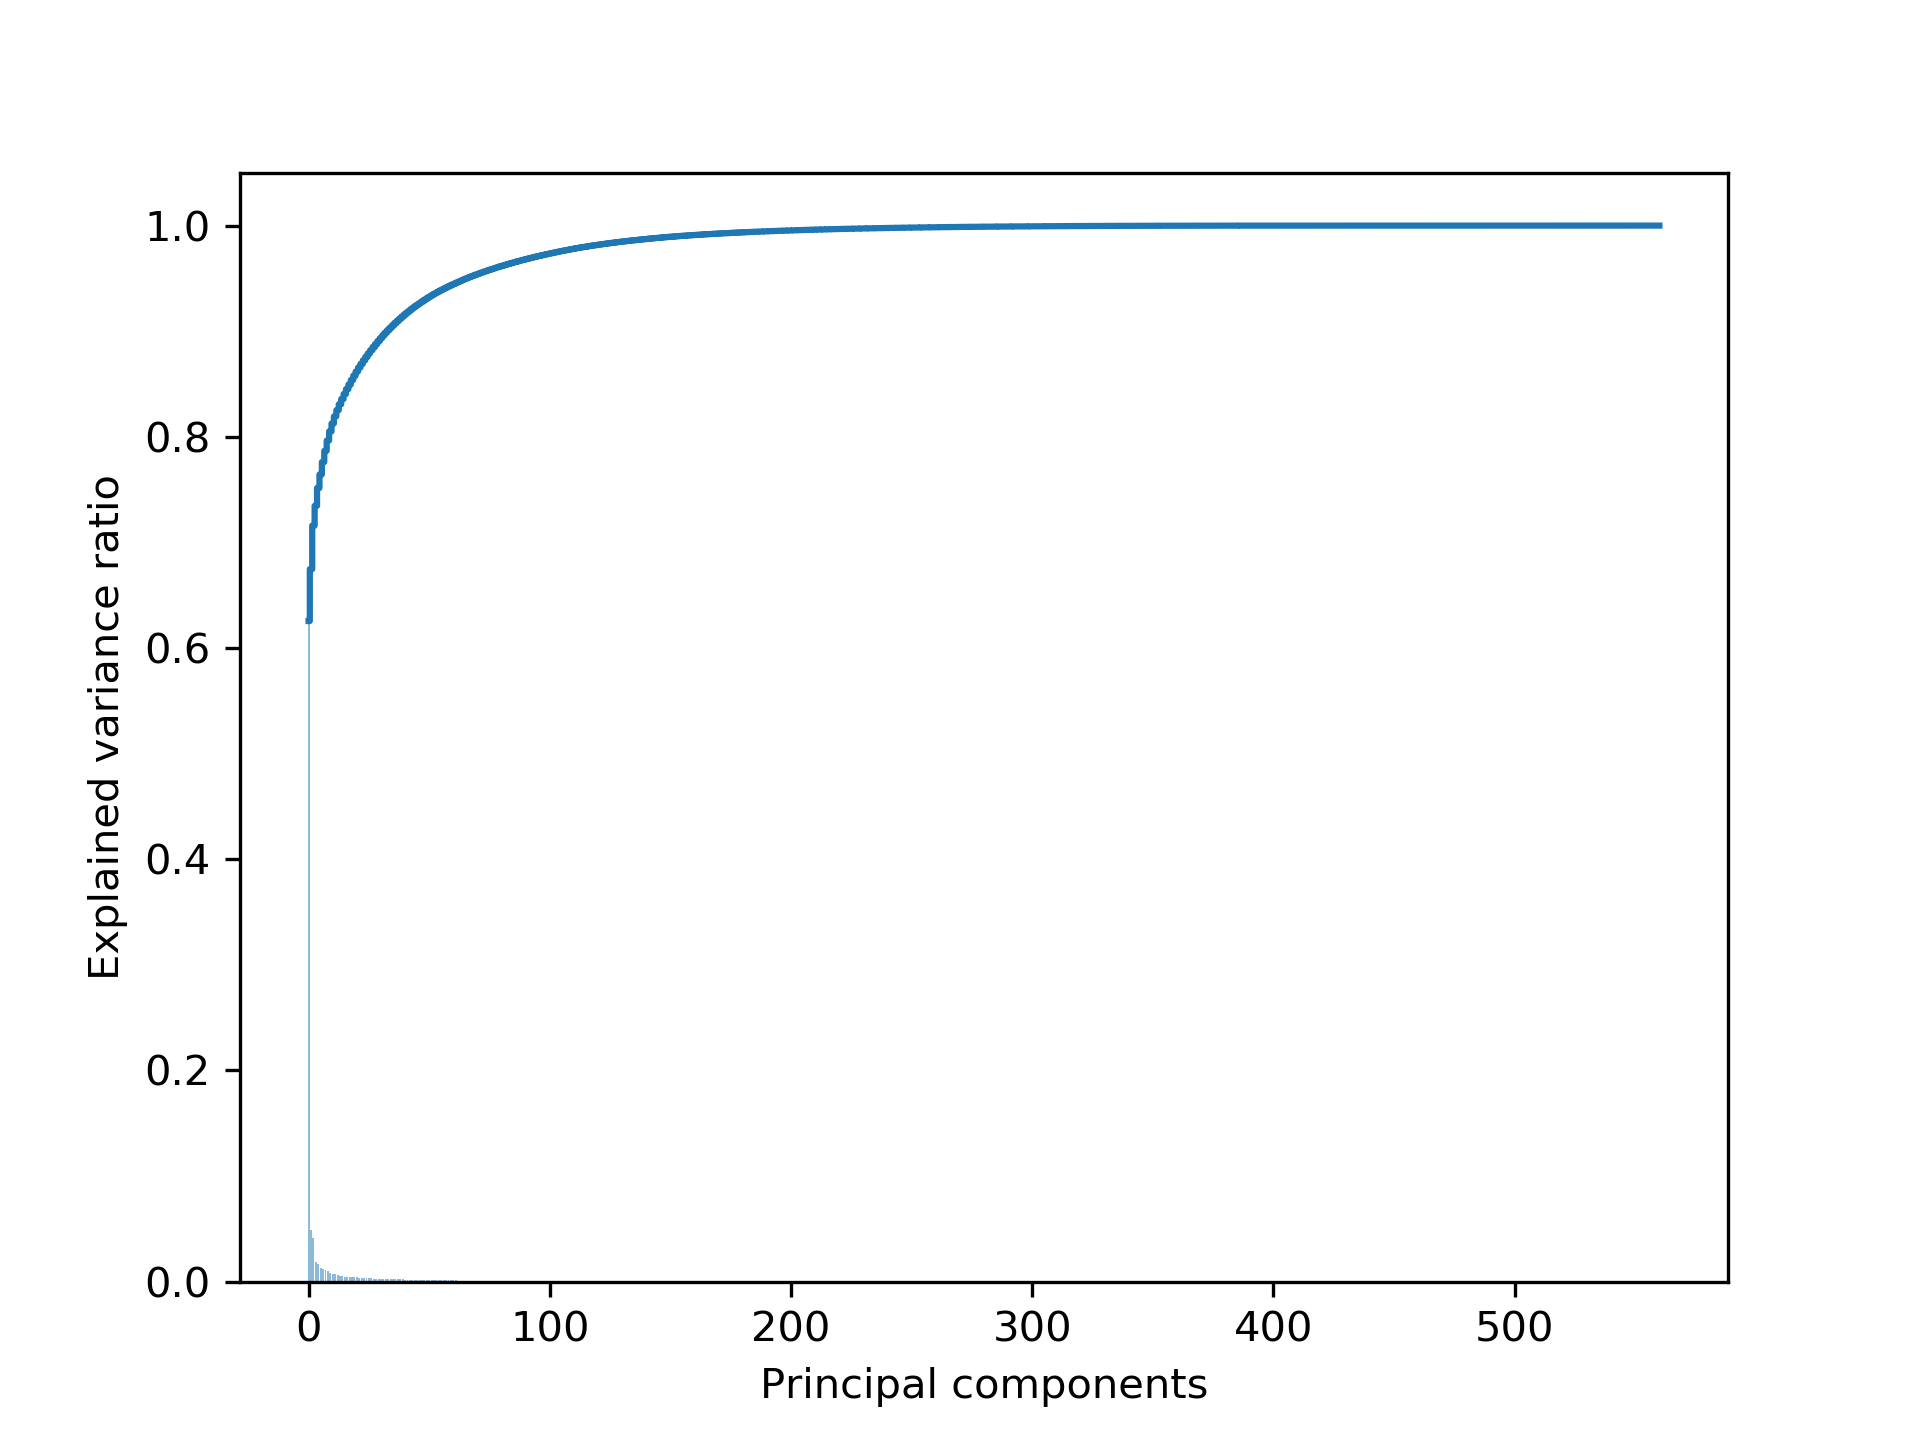
\includegraphics[width=\linewidth]{images/harpca.png}
    \caption{HAR Explained variance ratio.}\label{fig_harpca}
  \endminipage\hfill
  \minipage{0.32\textwidth}%
    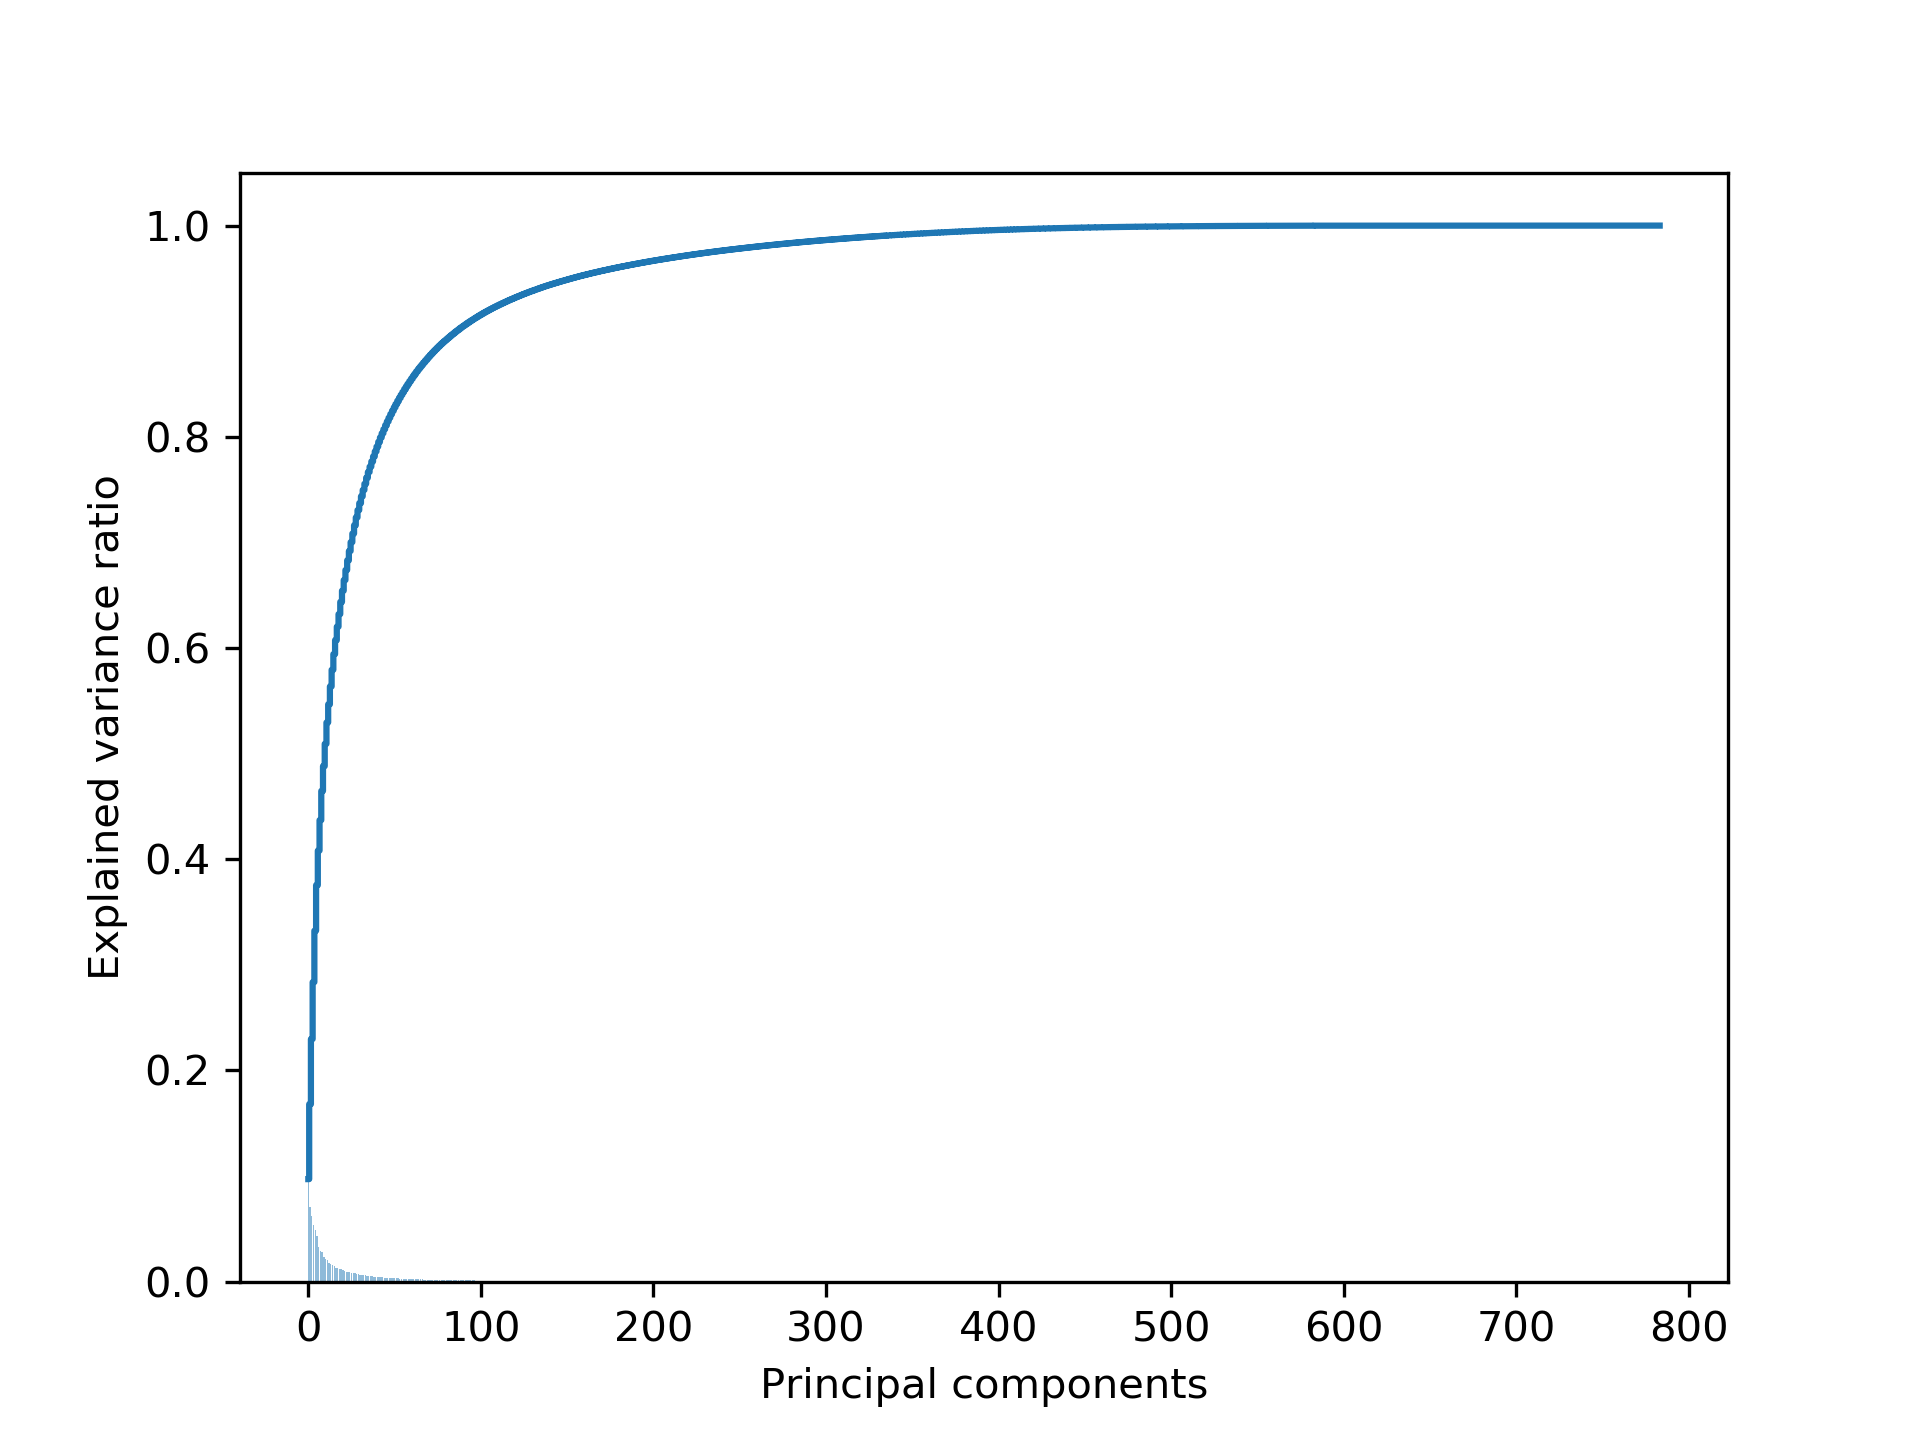
\includegraphics[width=\linewidth]{images/mnistpca.png}
    \caption{MNIST Explained variance ratio.}\label{fig_mnistpca}
  \endminipage
  \end{figure*}

\begin{figure*}[!htb]
  \minipage{0.32\textwidth}
    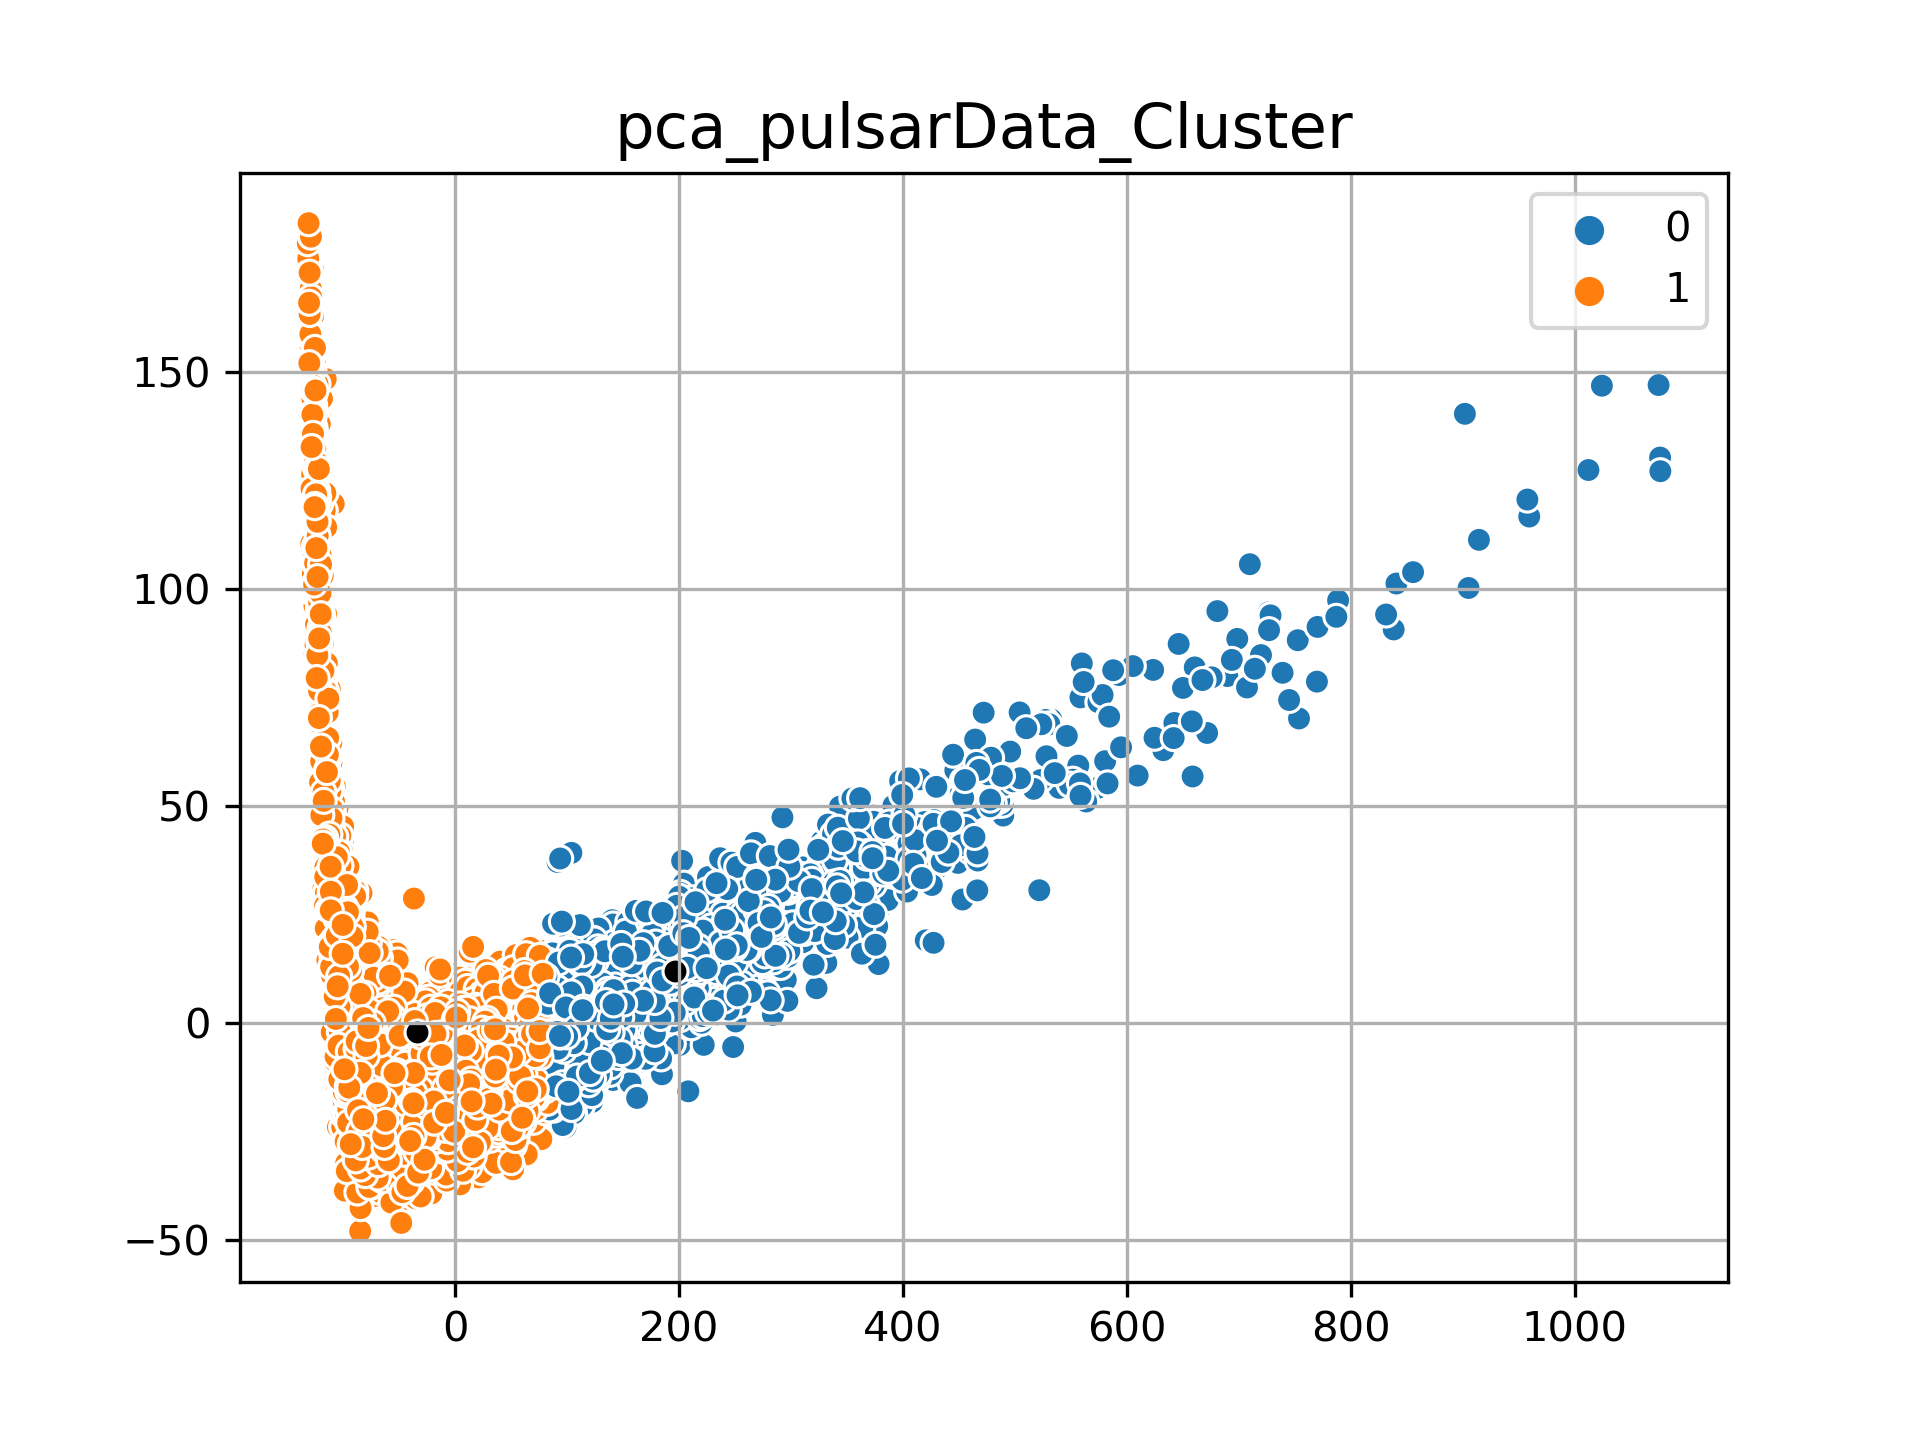
\includegraphics[width=\linewidth]{images/pca_pulsarData_Cluster.png}
    \caption{HTRU clustering after PCA.}\label{fig_pca_pulsarData_Cluster}
  \endminipage\hfill
  \minipage{0.32\textwidth}
    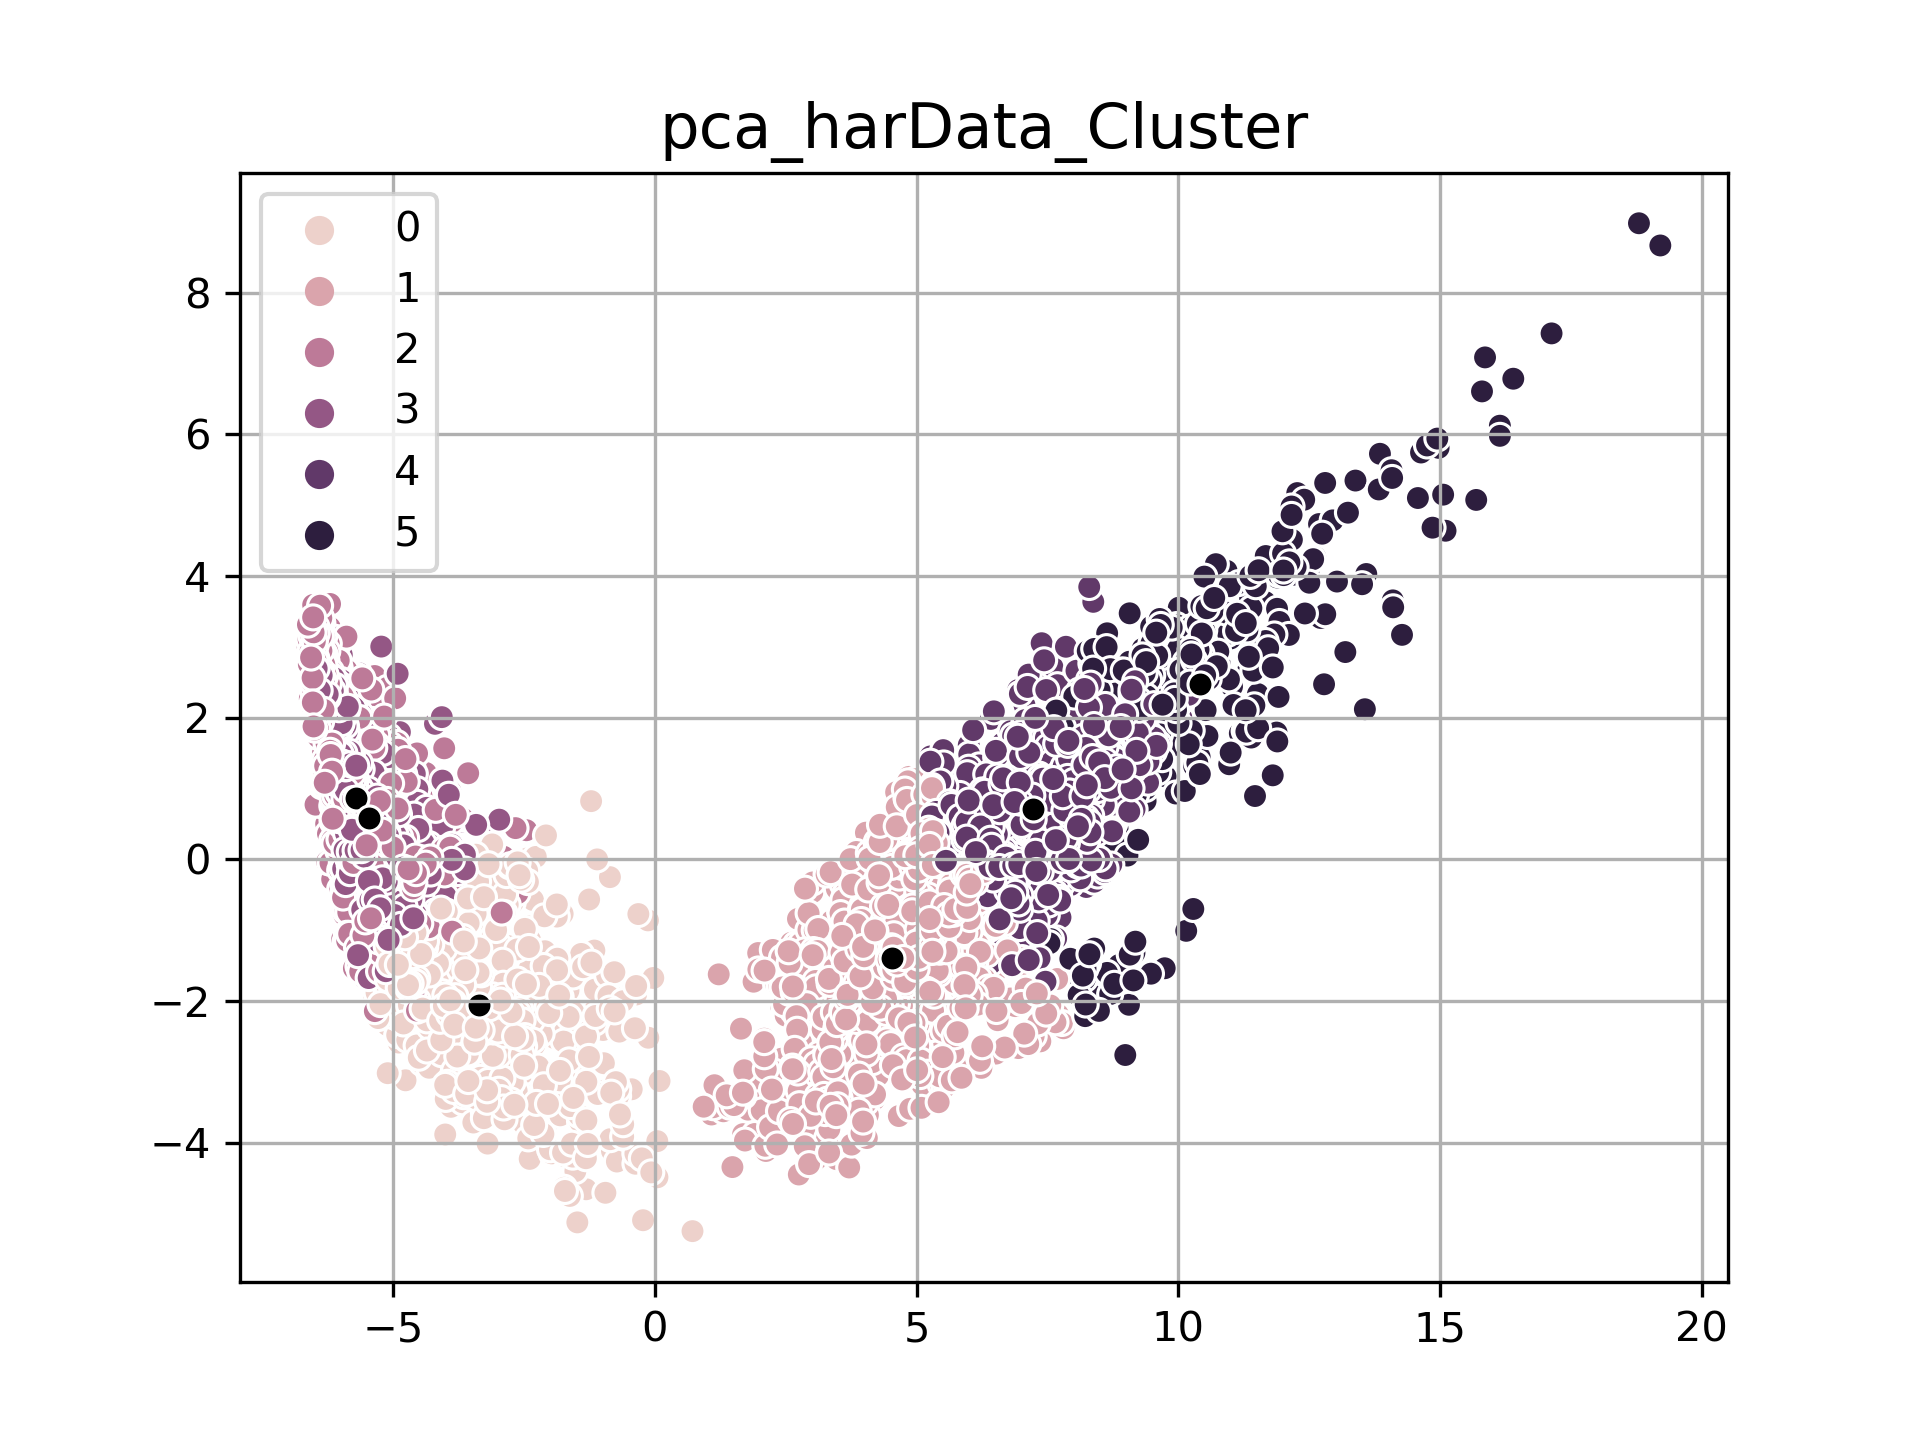
\includegraphics[width=\linewidth]{images/pca_harData_Cluster.png}
    \caption{HAR clustering after PCA}\label{fig_pca_harData_Cluster}
  \endminipage\hfill
  \minipage{0.32\textwidth}%
    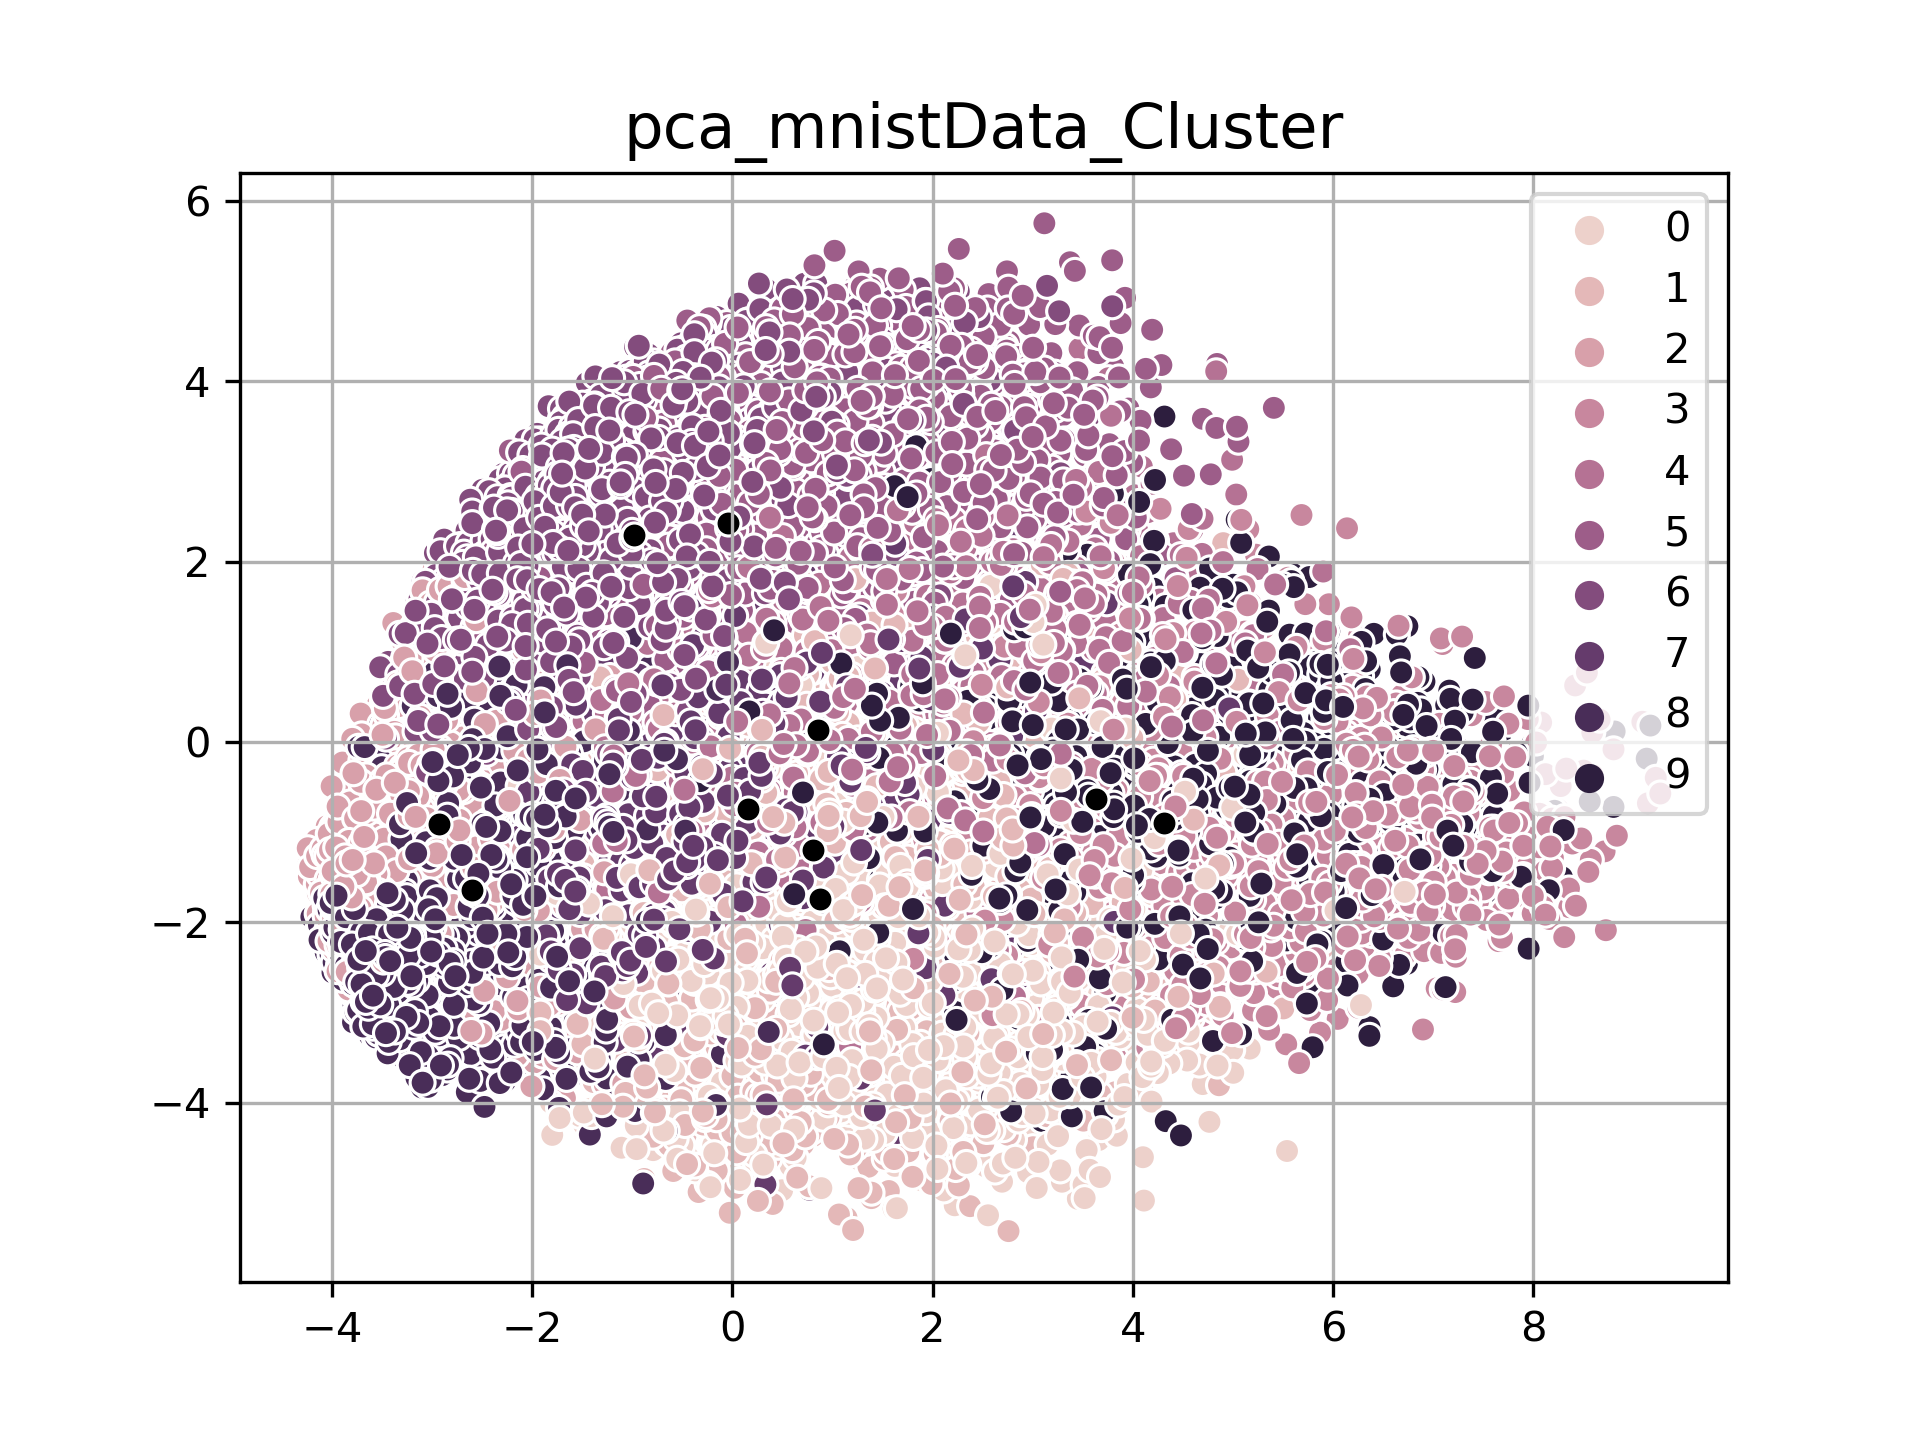
\includegraphics[width=\linewidth]{images/pca_mnistData_Cluster.png}
    \caption{MNIST clustering after PCA}\label{fig_pca_mnistData_Cluster}
  \endminipage
  \end{figure*}
  \begin{table*}[!ht]
    %% increase table row spacing, adjust to taste
    \renewcommand{\arraystretch}{1.3}
    % if using array.sty, it might be a good idea to tweak the value of
    % \extrarowheight as needed to properly center the text within the cells
    \caption{K-Means Clustering Results After PCA.}
    \label{tab_kmeans_pca_res}
    \centering
    \begin{tabular}{|c|c|c|c|c|c|}
    \hline
    Data - Method & Num. Components & Homogenity &  Completeness &  V-Measure &  Accuracy \\
    \hline
    \hline
    htru k-Means w/PCA &  4  &0.031206 &  2.302700e-02 &  2.649971e-02 &  0.765051 \\
    \hline
    har k-Means w/PCA&  200  & 0.570146 &  5.996766e-01 &  5.845388e-01 &  0.318961 \\
    \hline 
    mnist k-Means w/PCA& 400 & 0.486113 &  4.971782e-01 &  4.915831e-01 &  0.072782 \\
    \hline
    \end{tabular}
    \end{table*}

%In the core part of the clustering experiments, k-Means and DBSCAN algorithms will be used. These algorithms will be first compared to each other, then their results will be analyzed, evaluated and recorded for future comparisons. If there is enough time to deviate from the core path, agglomerative clustering algorithm will also be used, and these clustering algorithms will be tested again after applying dimensionality reduction methods like PCA/kernel PCA, LDA to the datasets. Given enough time, we will try these dimension reduction algorithms to confirm\cite{baldi1989neural}, in which it is concluded that the linear autoencoders with squared loss functions behave like PCAs. Otherwise, the experiments will continue with the autoencoders.  

\subsection{Feature Selection and Clustering}
\subsubsection{PCA}
For the feature selection, the first method we implemented was PCA. We transformed our data using the PCA function and retrieved the explained variance ratio to decide how many components we need. As it can be seen in figures 7,8 and 9, we choose the least amount of components representing almost all of the data.($\cong$0.99\%) As a result, we used 4 components for HTRU, 200 for HAR and 400 for MNIST and clustered the PCA reduced data using the k-Means algorithm. 
\par
\subsubsection{Linear AE}
After clustering with PCA, we implemented an end-to-end autoencoder with linear activation functions. The autoencoder has the basic structure shown in Figure 1. The input and output layers were set to the number of features of the datasets, and the latent feature layers were set to the same numbers we used in the PCA reduction. 'Adam' was used as the optimizer, and 'mean squared error' was used as the loss function. Finally, the batch size was set as 128, number of training epochs were set to 50 and our test sets were assigned as the validation data. \par
\subsubsection{Non-linear AE}
For the last feature selection method, we implemented the same autoencoder but replaced the linear activation function in the encoder model with a non-linear activation function, which is in this case was sigmoid. We also increased the number of training epochs for the non-linear case to 100. Previous number of training epochs was not enough for the non-linear autoencoder, which ended up as an underfitted model.

\begin{figure*}[!htb]
  \minipage{0.32\textwidth}
    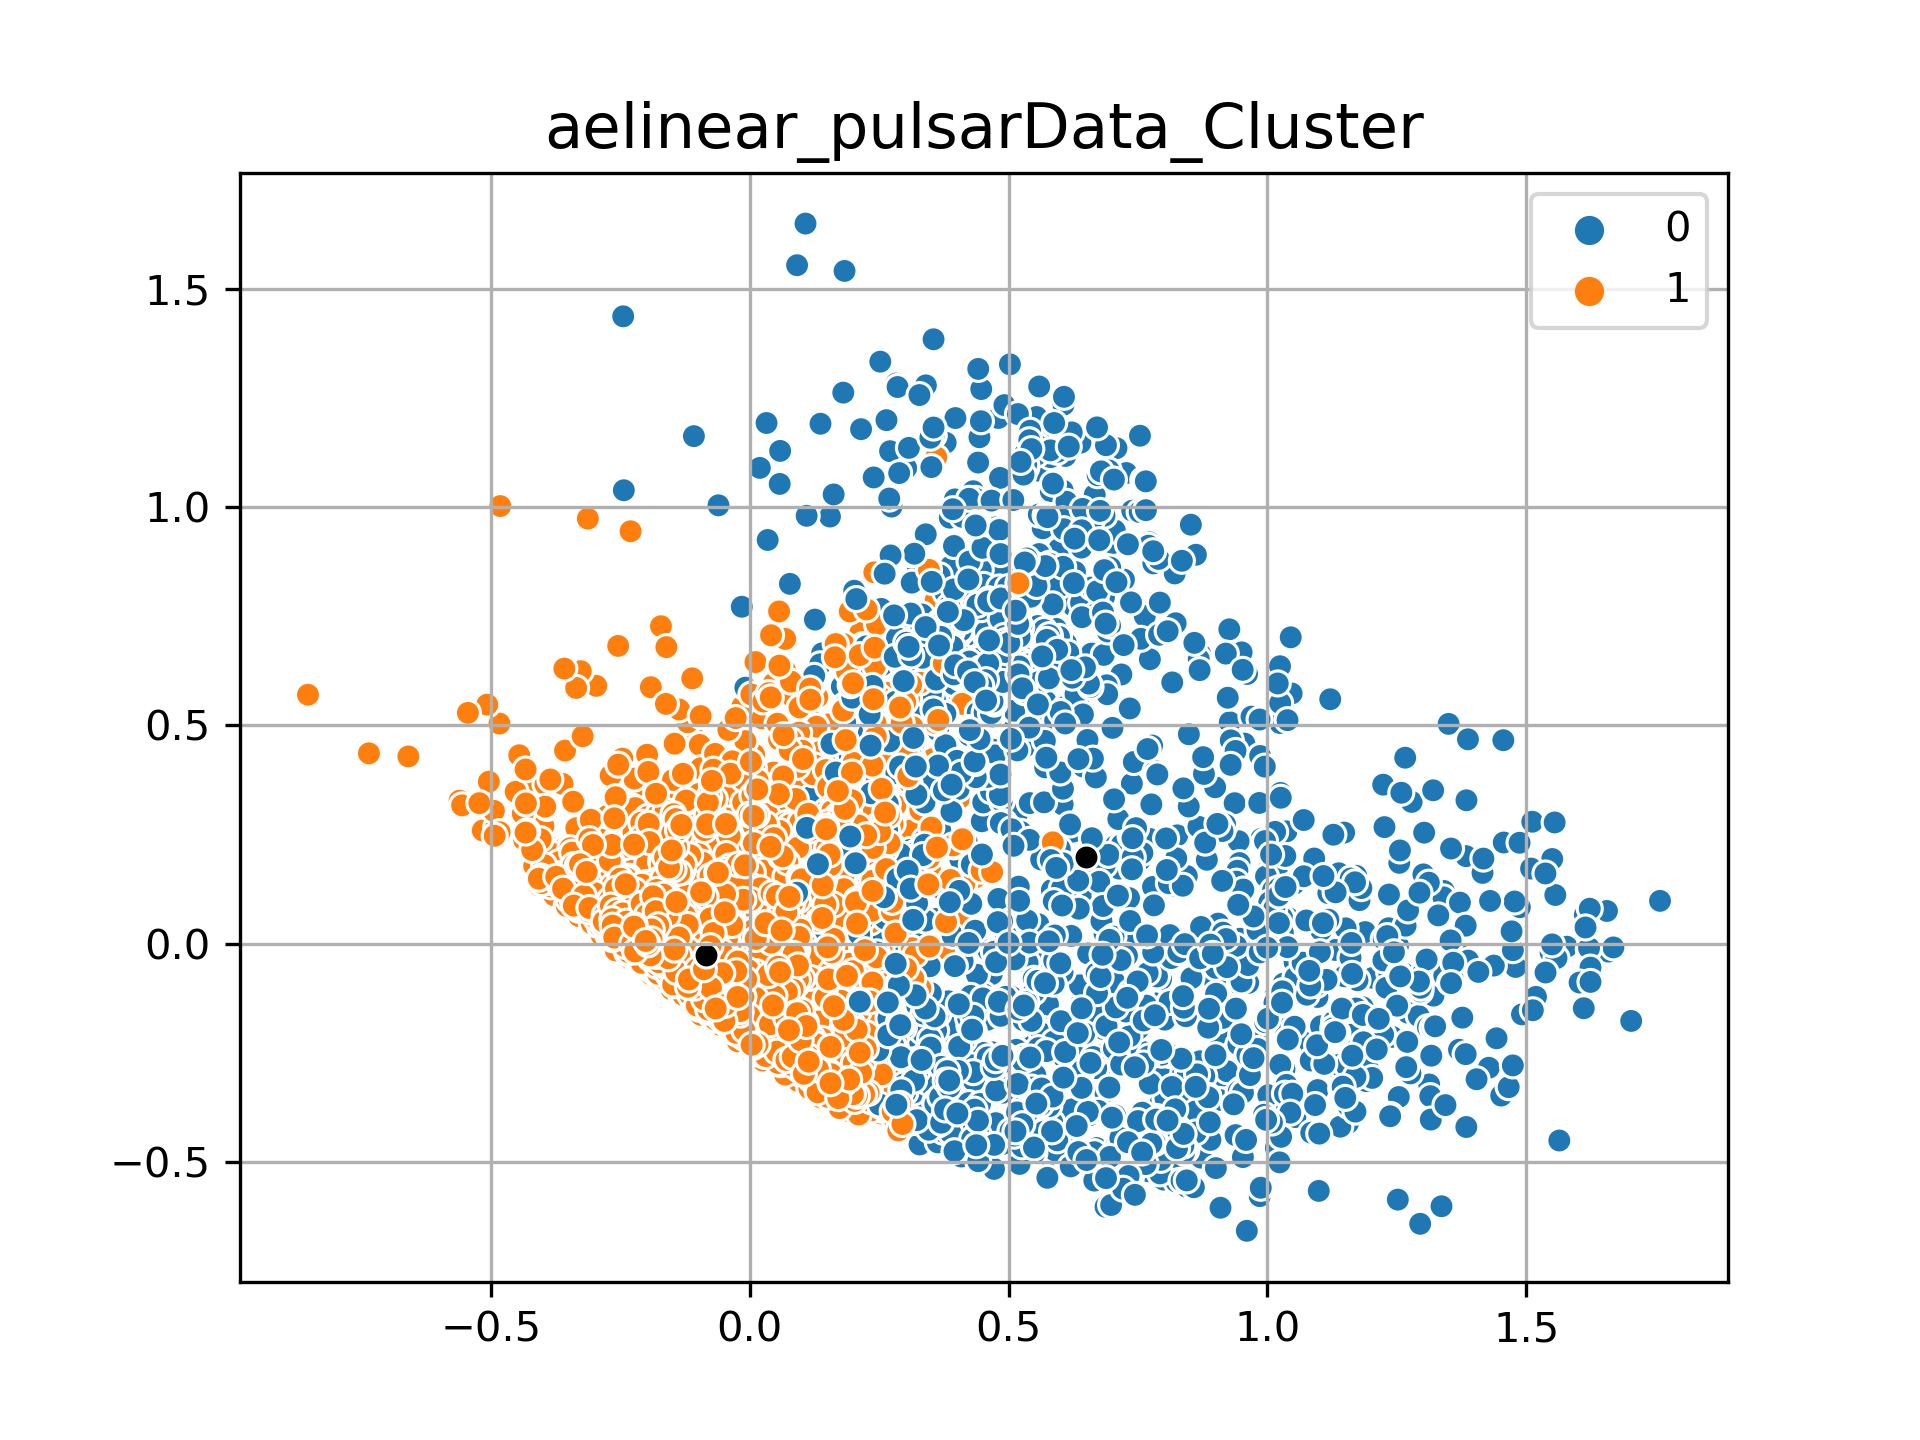
\includegraphics[width=\linewidth]{images/aelinear_pulsarData_Cluster.png}
    \caption{HTRU Explained variance ratio.}\label{fig_aelinear_pulsarData_Cluster}
  \endminipage\hfill
  \minipage{0.32\textwidth}
    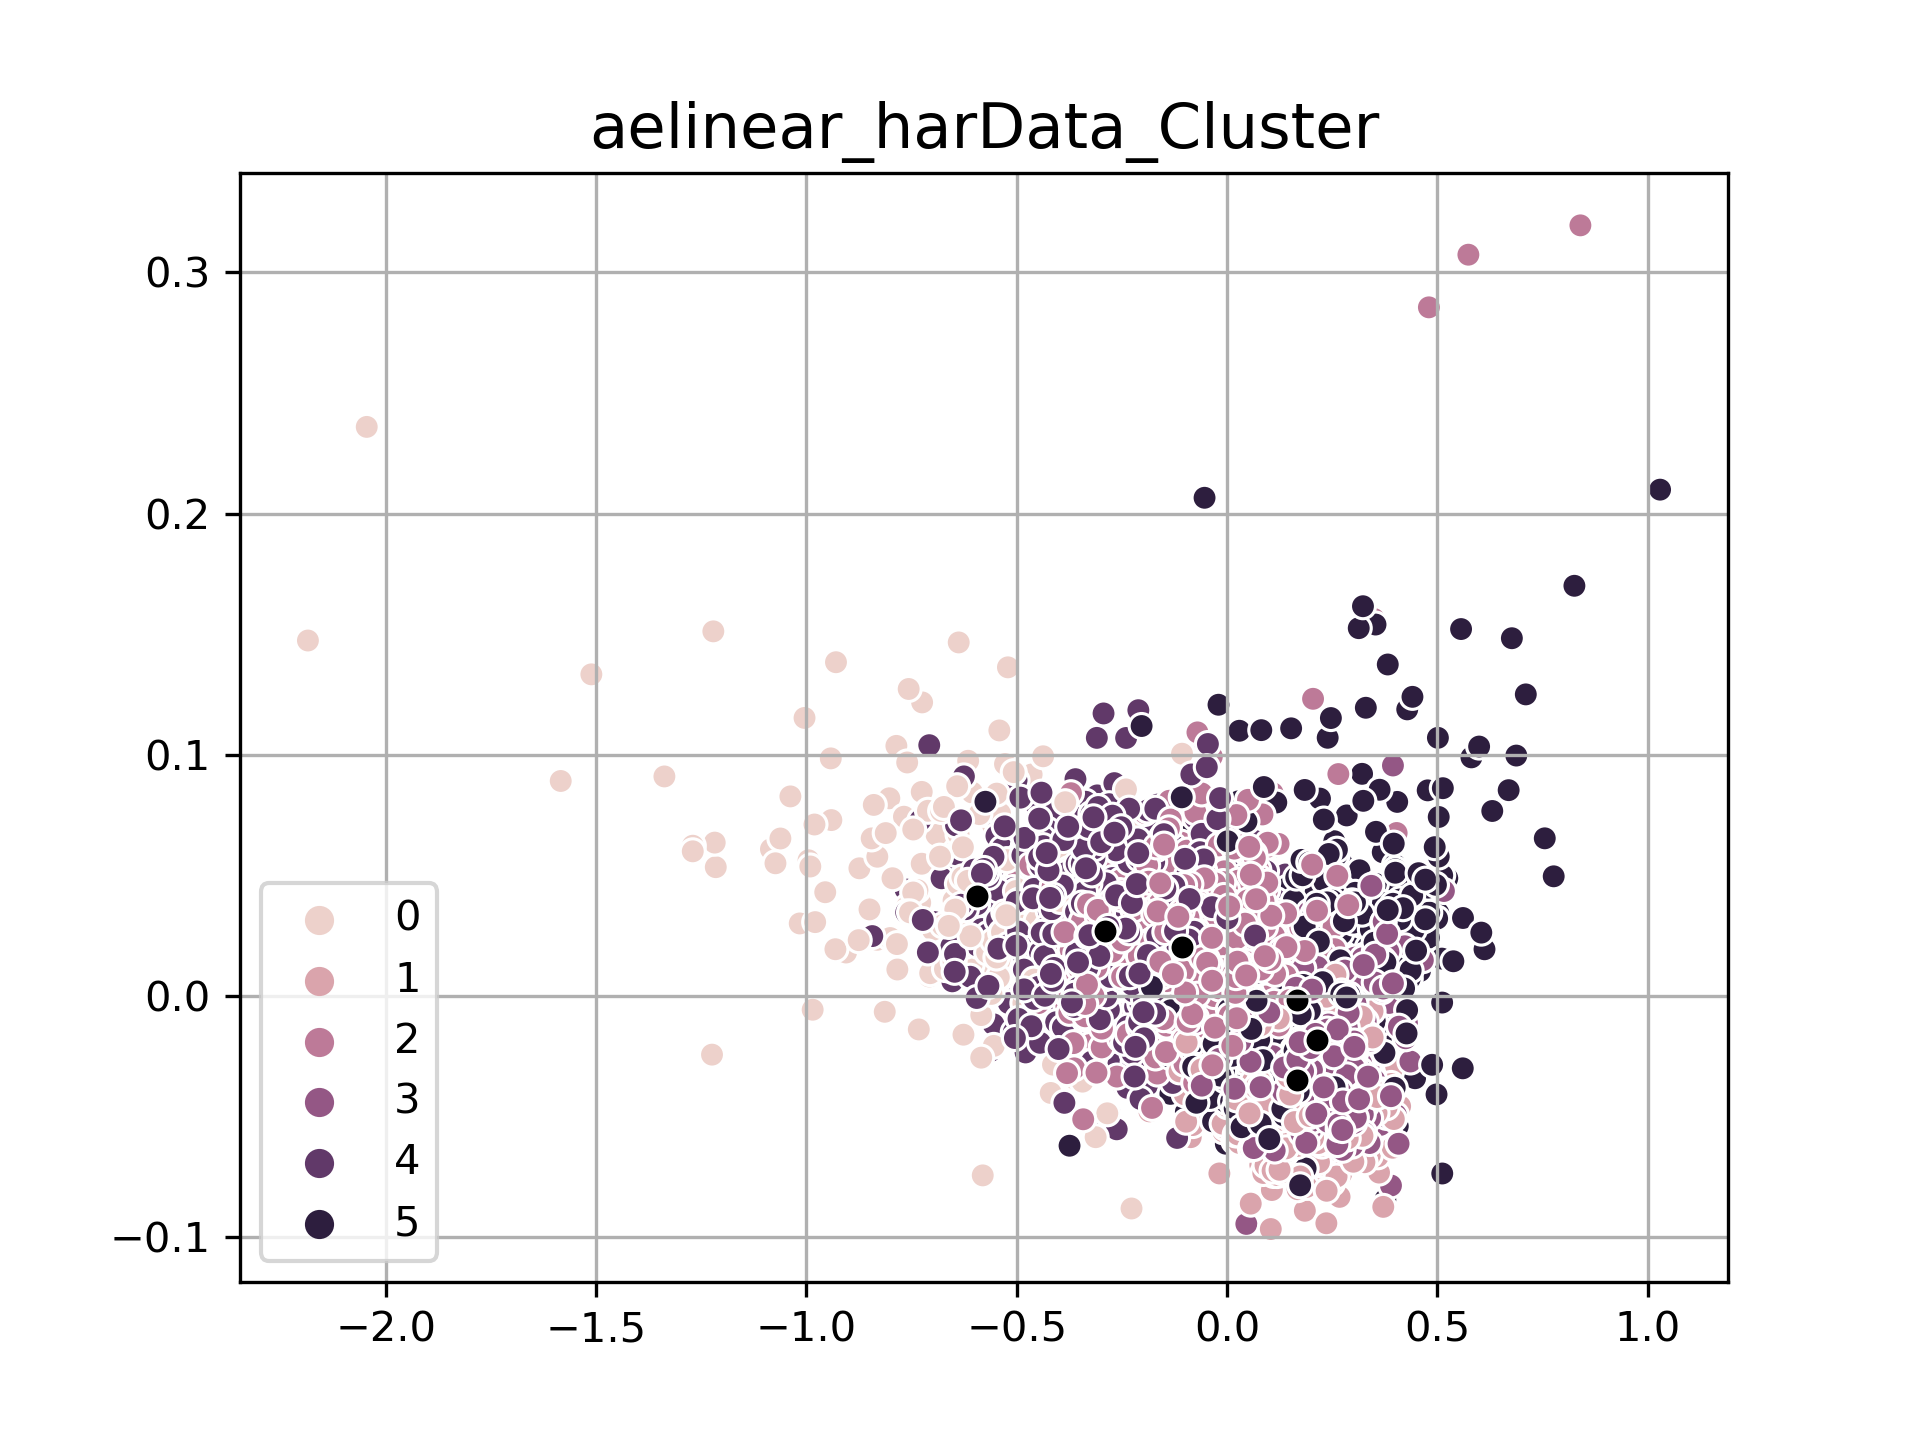
\includegraphics[width=\linewidth]{images/aelinear_harData_Cluster.png}
    \caption{HAR Explained variance ratio.}\label{fig_aelinear_harData_Cluster}
  \endminipage\hfill
  \minipage{0.32\textwidth}%
    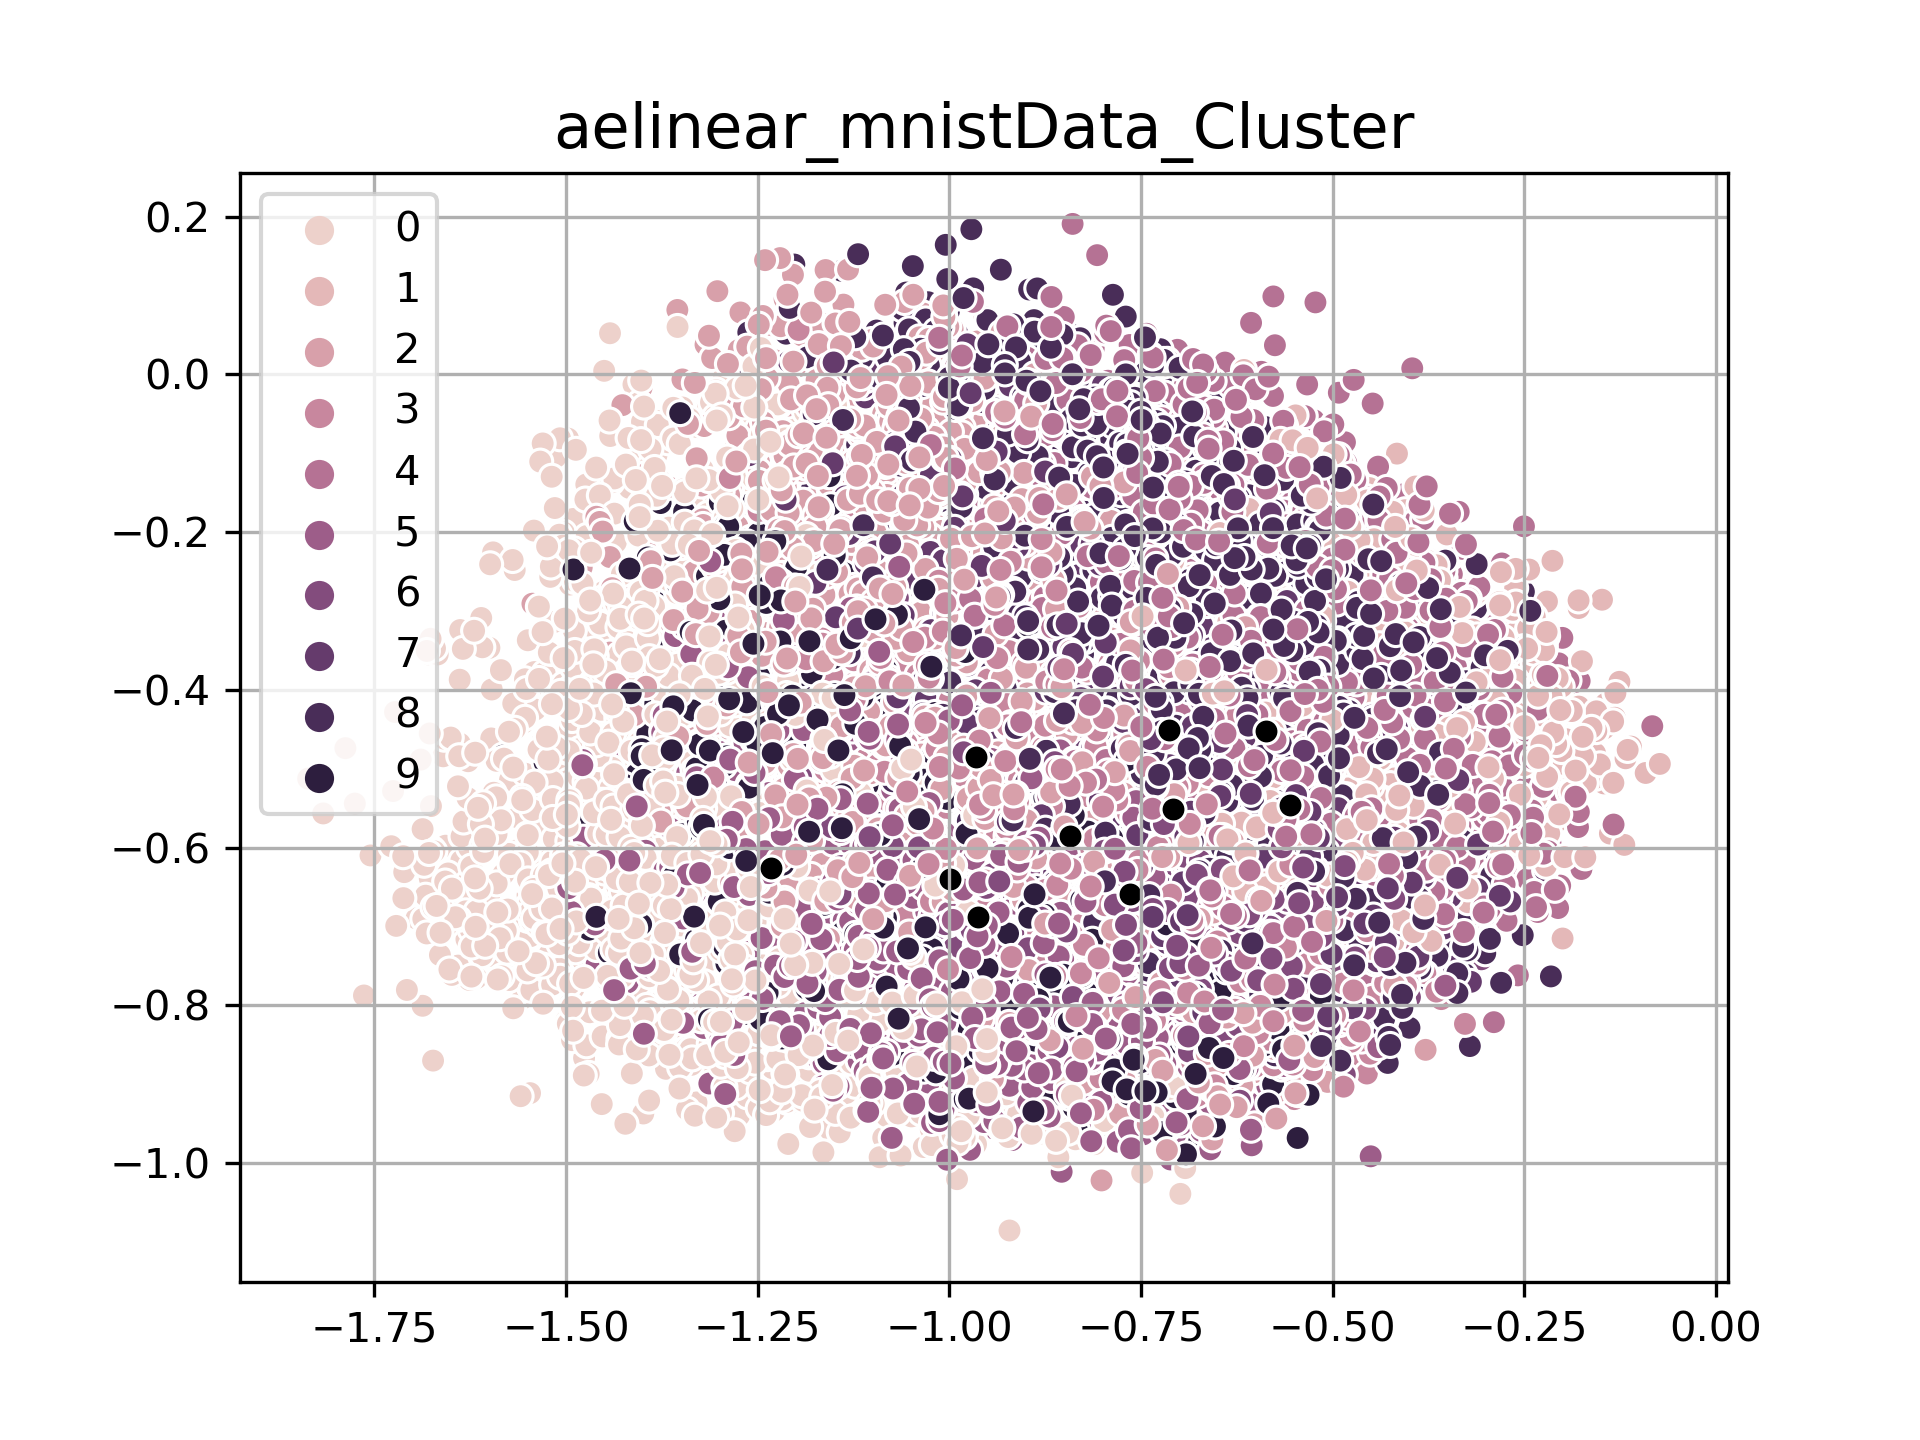
\includegraphics[width=\linewidth]{images/aelinear_mnistData_Cluster.png}
    \caption{MNIST Explained variance ratio.}\label{fig_aelinear_mnistData_Cluster}
  \endminipage
  \end{figure*}

\begin{figure*}[!htb]
  \minipage{0.32\textwidth}
    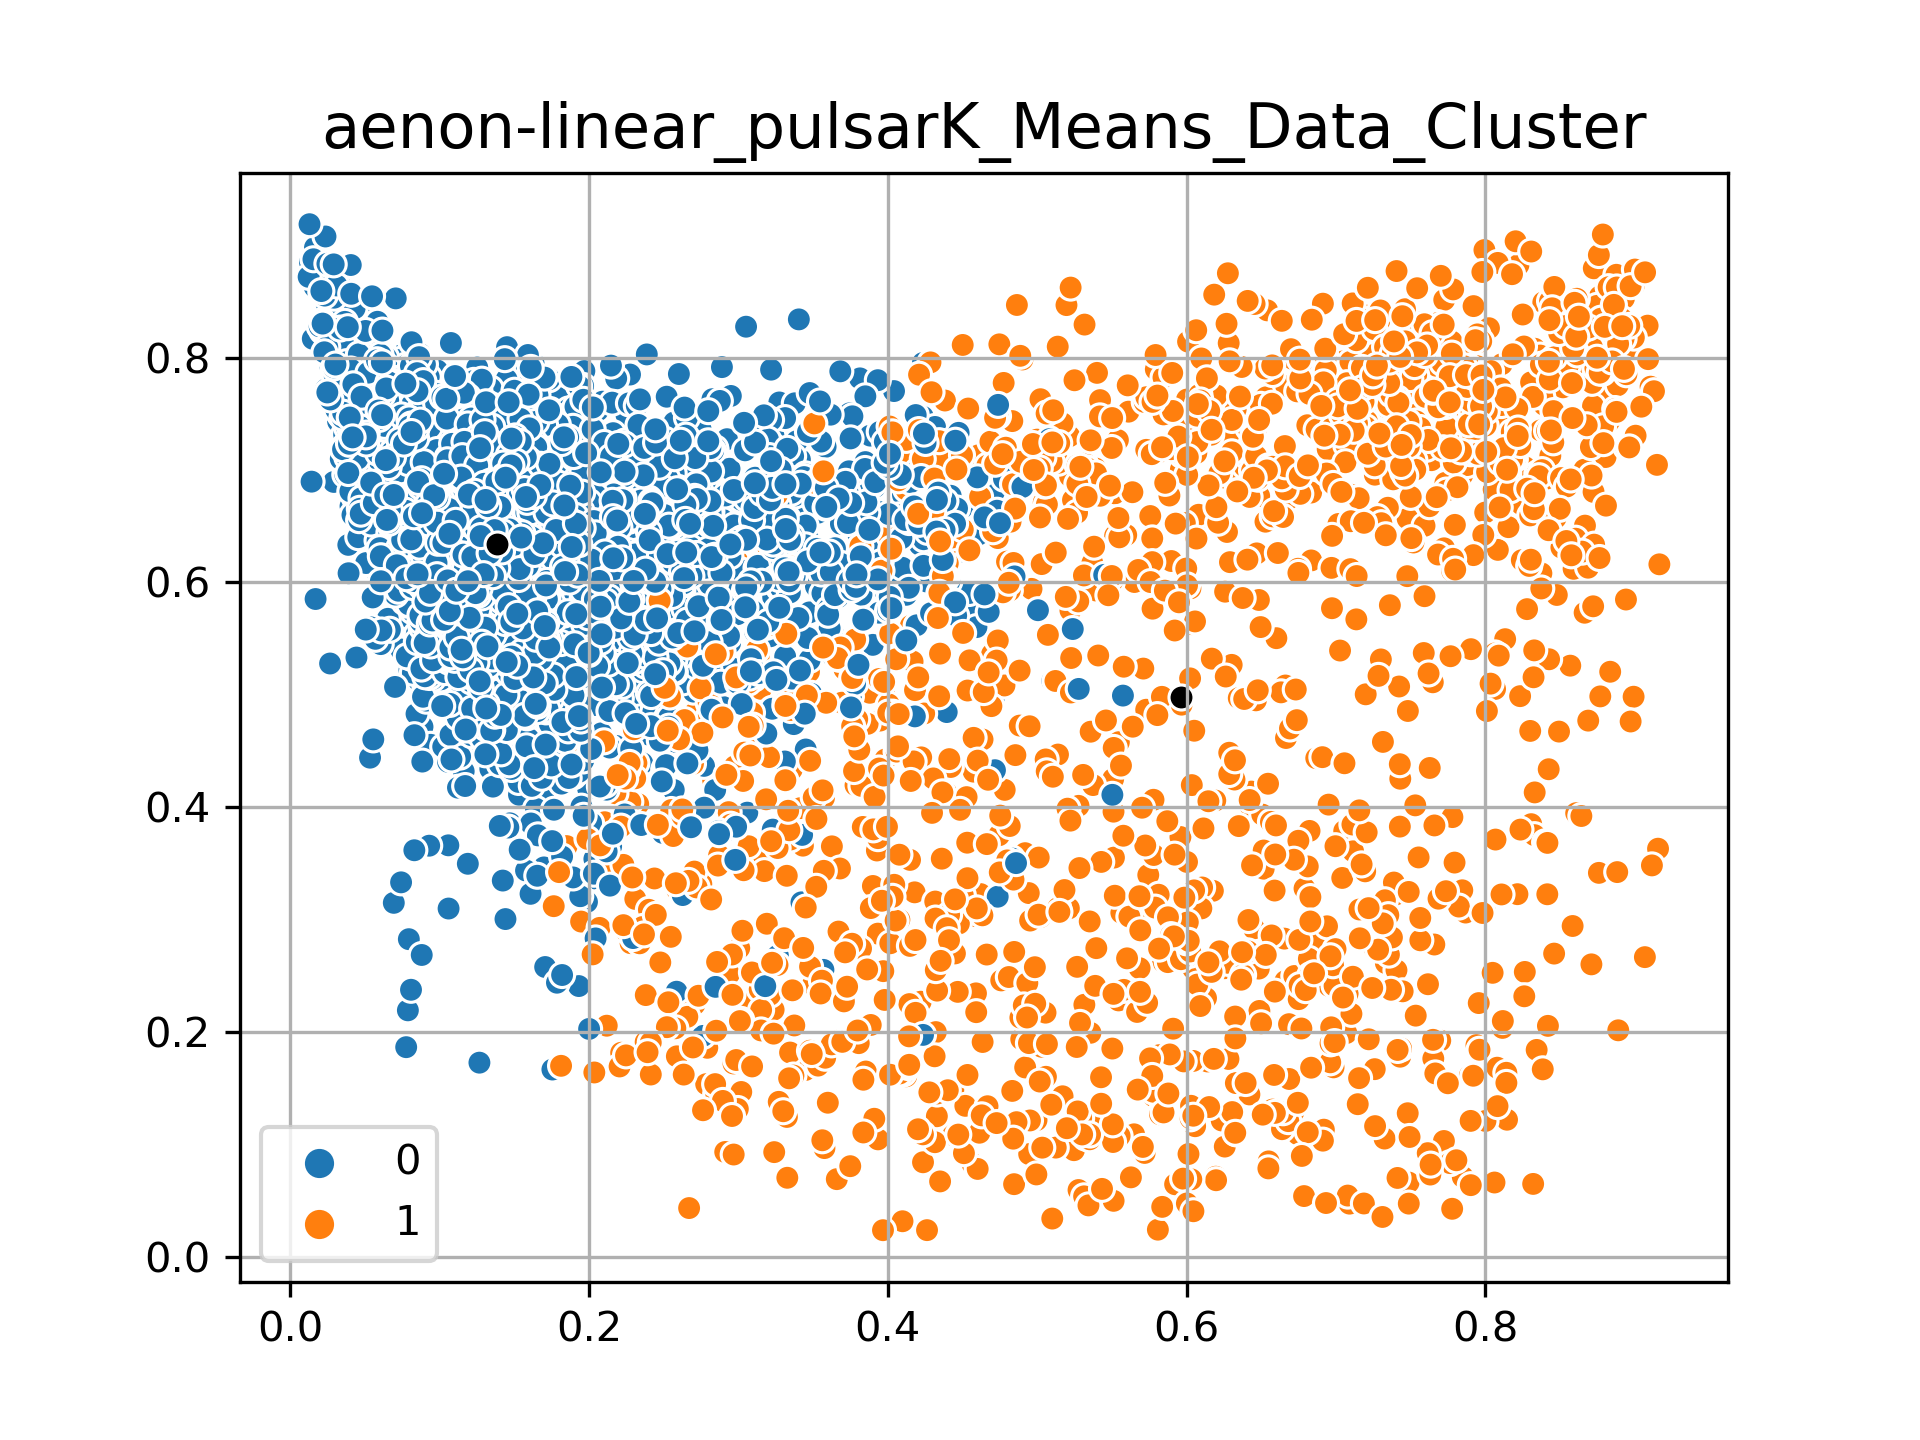
\includegraphics[width=\linewidth]{images/aenon-linear_pulsarK_Means_Data_Cluster.png}
    \caption{HTRU clustering after PCA.}\label{fig_linear_pulsarK_Means_Data_Cluster}
  \endminipage\hfill
  \minipage{0.32\textwidth}
    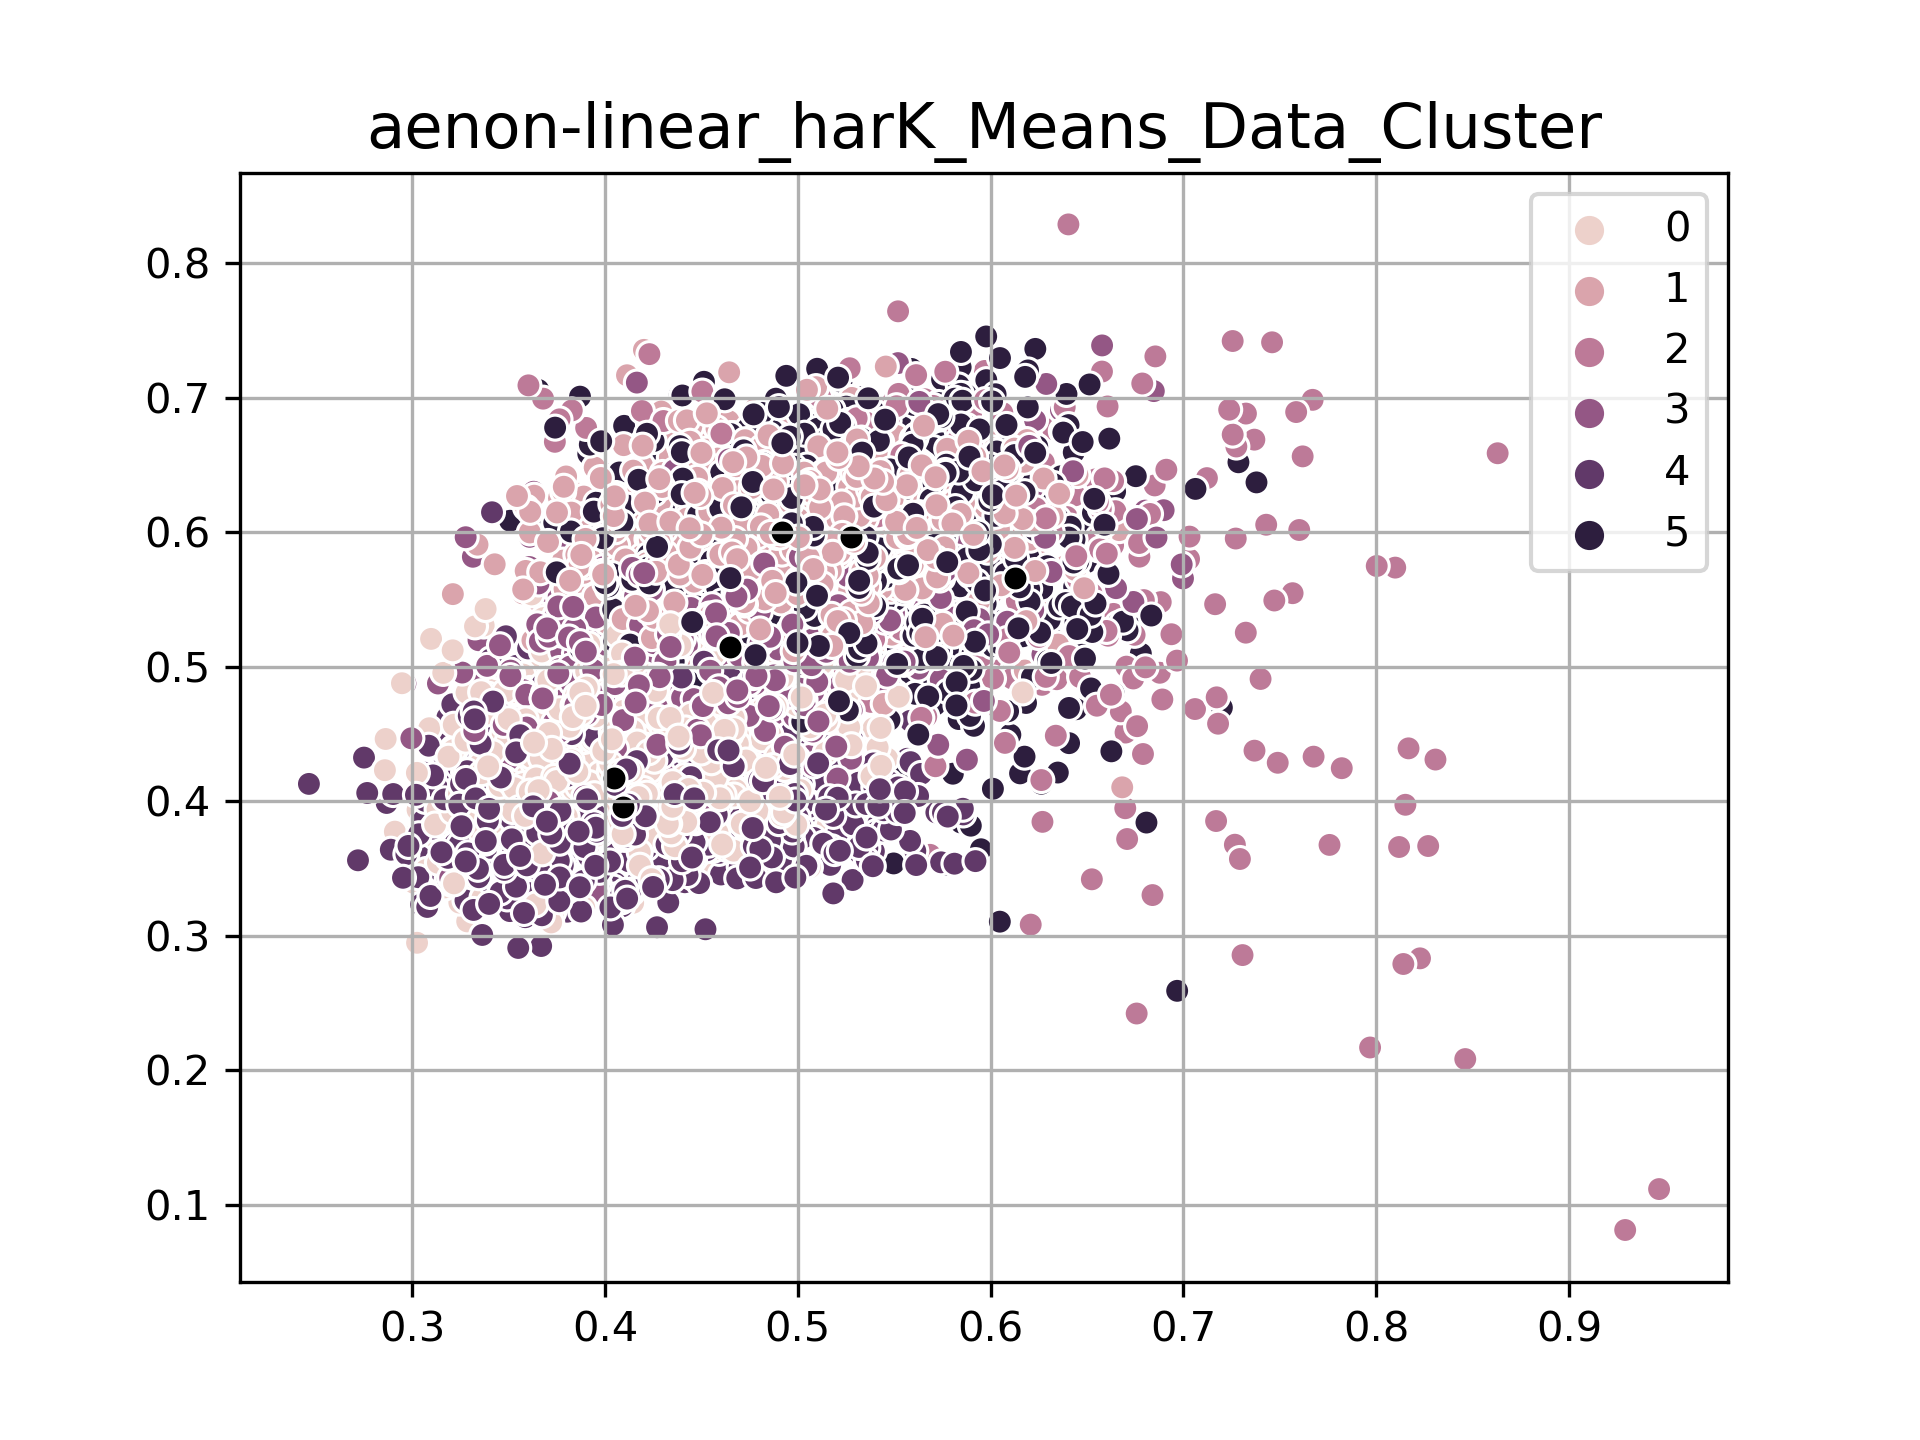
\includegraphics[width=\linewidth]{images/aenon-linear_harK_Means_Data_Cluster.png}
    \caption{HAR clustering after PCA}\label{fig_aenon-linear_harK_Means_Data_Cluster}
  \endminipage\hfill
  \minipage{0.32\textwidth}%
    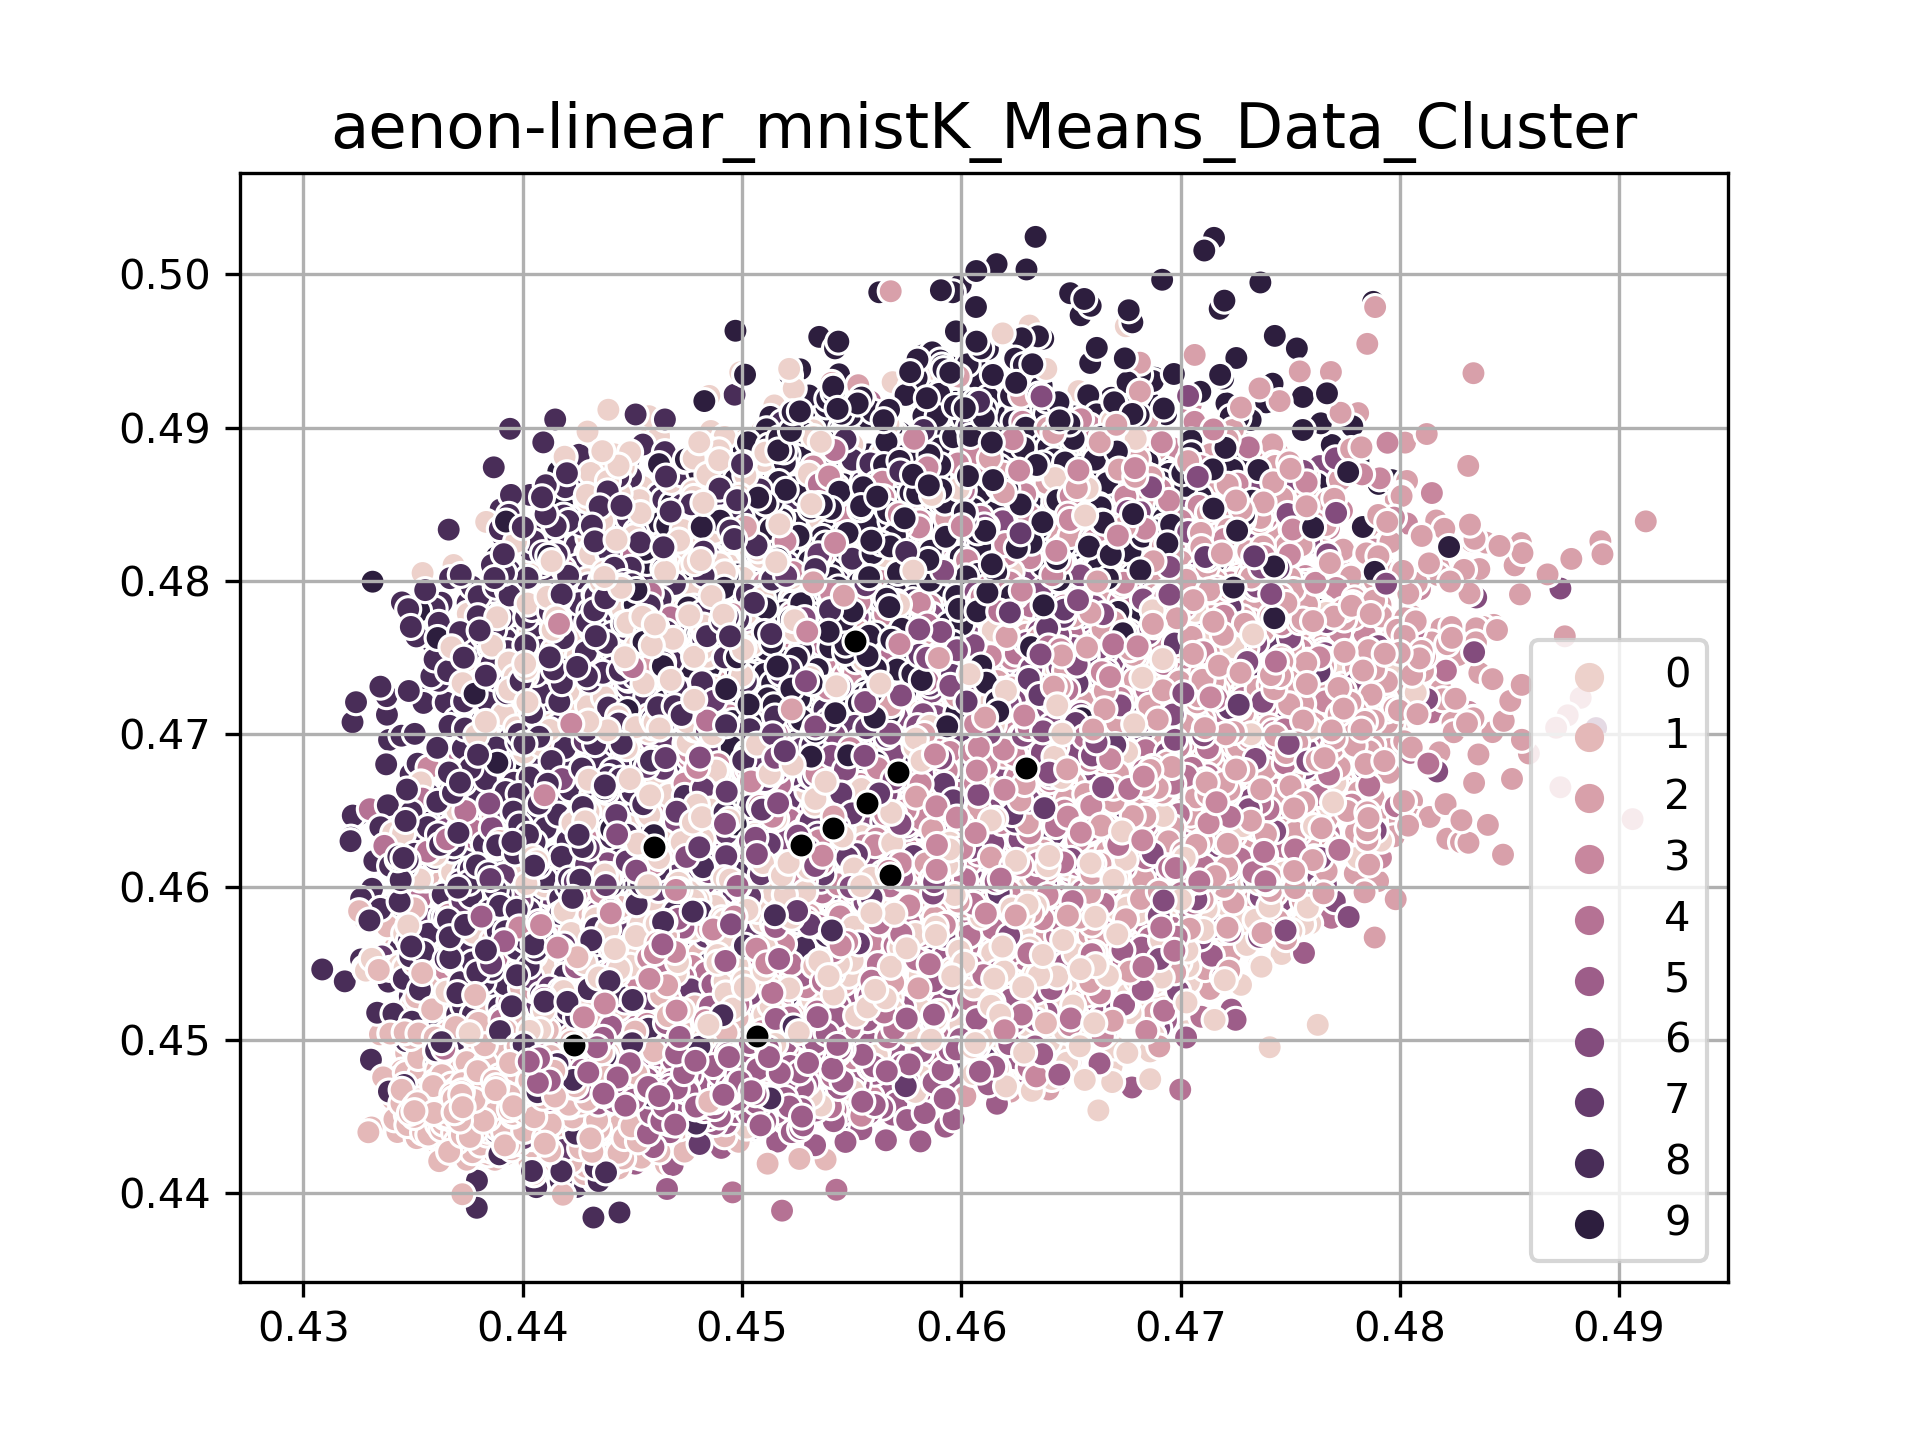
\includegraphics[width=\linewidth]{images/aenon-linear_mnistK_Means_Data_Cluster.png}
    \caption{MNIST clustering after PCA}\label{fig_aenon-linear_mnistK_Means_Data_Cluster}
  \endminipage
  \end{figure*}
  \begin{table*}[!ht]
    %% increase table row spacing, adjust to taste
    \renewcommand{\arraystretch}{1.3}
    % if using array.sty, it might be a good idea to tweak the value of
    % \extrarowheight as needed to properly center the text within the cells
    \caption{K-Means Clustering Results for linear and non-linear autoencoders.}
    \label{tab_lae_nlae}
    \centering
    \begin{tabular}{|c|c|c|c|c|c|}
    \hline
    Data - Method & Num. Latent Features & Homogenity &  Completeness &  V-Measure &  Accuracy \\
    \hline
    \hline
    htru k-Means w/LinAE &  4  &0.421208 &  3.674883e-01 &  3.925187e-01 &  0.935326 \\
    \hline
    har k-Means w/LinAE&  200  & 0.548367 &  5.951099e-01 &  5.707828e-01 &  0.180495 \\
    \hline 
    mnist k-Means w/LinAE& 400 & 0.247627 &  2.516646e-01 &  2.496297e-01 &  0.087673 \\
    \hline
    \hline
    htru k-Means w/N-LinAE &  4  &0.361558 &      0.312014 &   0.334964 &  0.925059 \\
    \hline
    har k-Means w/N-LinAE&  200  & 0.542958 &      0.574462 &   0.558266 &  0.184576 \\
    \hline 
    mnist k-Means w/N-LinAE& 400 & 0.493461 &      0.500976 &   0.497190 &  0.148200 \\
    \hline
    \end{tabular}
    \end{table*}
    \subsection{Softmax Clustering}
    In our final experiment, since our objective is to 'bin' our data into the softmax nodes; We created a new auto encoder with a softmax latent feature layer that has N nodes where N is the number of classes the given dataset has. Then for the output layer we followed \cite{xie2016unsupervised} and used Rectifier Linear Unit(ReLU) activation function, and we kept the rest of the network parameters same. After training the models, we separated each test set according to their class labels. Then we predicted each 'class-set' one by one to see which node played an active role in the clustering/binning of a given class sample. Finally, as it can be seen in the Table 5, if the classes of a given set was binned properly, we made the assumption that the model was trained correctly and evaluated the scores on all of the test set. The results presented here only show the nodes that best cluster a given class-set, excluding the HTRU set because it only has two classes. Complete class versus node accuracy tables can be found in the Appendix. 

\begin{table}[!ht]
  %% increase table row spacing, adjust to taste
  \renewcommand{\arraystretch}{1.3}
  % if using array.sty, it might be a good idea to tweak the value of
  % \extrarowheight as needed to properly center the text within the cells
  \caption{HTRU Softmax Results.}
  \label{tab_htru_sfx}
  \centering
  \begin{tabular}{|c|c|c|}
  \hline
  Class vs. Output Node Accuracy& Node 0 & Node 1  \\
  \hline
  \hline
  Class 0   &  \textbf{0.9963}    & 0.00368 \\
  \hline
  Class 1   &  0.26168  &  \textbf{0.73831} \\
  \hline
  \multicolumn{2}{|c|}{HTRU Test Accuracy:  } & 0.973184\\
  \hline  

\end{tabular}
  \end{table}

  \begin{table}[!ht]
    %% increase table row spacing, adjust to taste
    \renewcommand{\arraystretch}{1.3}
    % if using array.sty, it might be a good idea to tweak the value of
    % \extrarowheight as needed to properly center the text within the cells
    \caption{HAR Softmax Results.}
    \label{tab_har_sfx}
    \centering
    \begin{tabular}{|c|c|c|c|c|c|c|}
    \hline
    Class vs. Output Node Accuracy & Node 3 & Node 4 & Node 5\\
    \hline
    \hline
    Class 0    & 0.131  &  0.004    & \textbf{0.77}\\
    \hline
    Class 1    & 0.00  &  \textbf{0.513}    & 0.377\\
    \hline
    Class 2   & 0.009  &  0.007    & \textbf{0.704}\\
    \hline
    Class 3   & \textbf{0.847}  &  0.0    & 0.0\\
    \hline
    Class 4  & \textbf{0.874 } &  0.0    & 0.0\\
    \hline
    Class 5    & \textbf{0.774  }&  0.0    & 0.0\\
    \hline
    \end{tabular}
    \end{table}
    \begin{table}
      %% increase table row spacing, adjust to taste
      \renewcommand{\arraystretch}{1.3}
      % if using array.sty, it might be a good idea to tweak the value of
      % \extrarowheight as needed to properly center the text within the cells
      \caption{HAR Softmax Results.}
      \label{tab_har_sfx_all}
      \centering
      \begin{tabular}{|c|c|}
      \hline
      Class vs. Output Node Accuracy & Node 0 \\
      \hline
      \hline
      Class 0   &  \textbf{1.0}   \\
      \hline
      Class 1   &  \textbf{1.0}   \\
      \hline
      Class 2   &  \textbf{1.0}   \\
      \hline
      Class 3   &  \textbf{1.0}  \\
      \hline
      Class 4   &  \textbf{1.0}  \\
      \hline
      Class 5   &  \textbf{1.0}  \\
      \hline
      Class 6   &  \textbf{1.0}   \\
      \hline
      Class 7   &  \textbf{1.0}  \\
      \hline
      Class 8   &  \textbf{1.0}  \\
      \hline
      Class 9   &  \textbf{1.0}  \\
      \hline
      \end{tabular}
      \end{table}
\section{Discussion}

Evaluation of the experiments in which we use k-Means, were done using scikit-learn metrics library. For each experiment completeness, homogeneity, v-measure and accuracy scores were calculated.\par
When we look at the results, we can clearly see that the k-Means algorithm with feature selection performs much better than our baseline clustering. But comparing the feature selection methods is complicated. If we look at PCA and linear autoencoder, their results were usually similar but differences could still be observed. And this point brings us back to \cite{hinton2006reducing}. Even though PCA is a robust algorithm, autoencoders are not and they can be difficult to train. Then, when we look at non-linear autoencoders, it is mostly an improvement over the other methods. Especially the performance increase on a complex dataset like MNIST is great. In the end we believe that if we need to extract good features, we should start with simple and robust methods like PCA and try more complex methods like autoencoders if the former does not help.\par

For the softmax clustering part, evaluation was not as straightforward as the first part. Because when we try to cluster our data- even if we assume that it can cluster the data perfectly- we need to find out which output node clusters which class of the data. But this is a very strong assumption. Since we do not have any control over how the hidden softmax layer learns to represent the data while training, we can end up with endless combinations of possible representations. We can see this problem occuring in the results of the HAR and MNIST datasets. However, the results we got for the HTRU dataset was surprisingly good, and when we repeated the experiment our results were consistent most of the time. We believe the success of the HTRU dataset is related to its small amount of features and classes. In the future, we will definitely try different datasets that are a little bit  larger than HTRU and compare it to our results.\par
The prediction and evaluation procedure we follow can be seen in Figure 19. After we predict the class-sets and apply argmax function to the resulting array, we end up with the indices of the nodes. Then, we calculate the accuracy score of the node index array compared to the class-set labels, which are just arrays filled with their own class labels. After calculating the accuracy for every class-set label, we end up with a distribution that shows how much of the predicted class-set is clustered by which output node.  
\begin{figure}[!htb]
  
    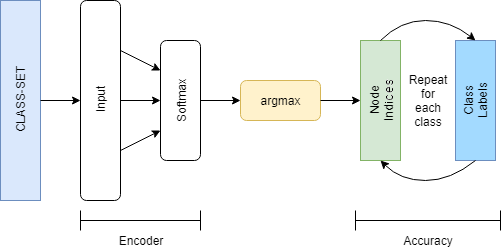
\includegraphics[width=\linewidth]{images/Model.png}
    \caption{Prediction and node-class accuracy calculation process.}\label{fig_model}
 
  \end{figure}

\section{Conclusion}

We briefly explained the purpose and the tasks of the project, and presented our results. While going through the literature, importance of unsupervised learning was understood. Also, it was realized that the field needs more attention. Later on, we described our model and the datasets we used. Then the experiments we have done were explained in detail. Finally, analyzed and discussed our results.
\newpage 

% if have a single appendix:
%\appendix[Proof of the Zonklar Equations]
% or
%\appendix  % for no appendix heading
% do not use \section anymore after \appendix, only \section*
% is possibly needed

% use appendices with more than one appendix
% then use \section to start each appendix
% you must declare a \section before using any
% \subsection or using \label (\appendices by itself
% starts a section numbered zero.)
%



% you can choose not to have a title for an appendix
% if you want by leaving the argument blank



% trigger a \newpage just before the given reference
% number - used to balance the columns on the last page
% adjust value as needed - may need to be readjusted if
% the document is modified later
%\IEEEtriggeratref{8}
% The "triggered" command can be changed if desired:
%\IEEEtriggercmd{\enlargethispage{-5in}}

% references section

% can use a bibliography generated by BibTeX as a .bbl file
% BibTeX documentation can be easily obtained at:
% http://mirror.ctan.org/biblio/bibtex/contrib/doc/
% The IEEEtran BibTeX style support page is at:
% http://www.michaelshell.org/tex/ieeetran/bibtex/

\bibliographystyle{IEEEtran}

\bibliography{refs}
\newpage
\appendix[Full Tables]
See page 8.
  \begin{table*}
    %% increase table row spacing, adjust to taste
    \renewcommand{\arraystretch}{1.3}
    % if using array.sty, it might be a good idea to tweak the value of
    % \extrarowheight as needed to properly center the text within the cells
    \caption{HAR Softmax Clustering Results.}
    \label{tab_har_sfx_all}
    \centering
    \begin{tabular}{|c|c|c|c|c|c|c|}
    \hline
    Class vs. Output Node Accuracy & Node 0 & Node 1 & Node 2 & Node 3 & Node 4 & Node 5\\
    \hline
    \hline
    Class 0   &  0.0    & 0.086 &  0.0    & 0.131  &  0.004    & \textbf{0.77}\\
    \hline
    Class 1   &  0.0  &  0.006 &  0.10    & 0.00  &  \textbf{0.513}    & 0.377\\
    \hline
    Class 2   &  0.0    & 0.24 &  0.038    & 0.009  &  0.007    & \textbf{0.704}\\
    \hline
    Class 3   &  0.0  &  0.0 &  0.152    & \textbf{0.847}  &  0.0    & 0.0\\
    \hline
    Class 4   &  0.0   & 0.0 &  0.125    & \textbf{0.874 } &  0.0    & 0.0\\
    \hline
    Class 5   &  0.0  &  0.0&  0.225    & \textbf{0.774  }&  0.0    & 0.0\\
    \hline
    \end{tabular}
    \end{table*}

    \begin{table*}
      %% increase table row spacing, adjust to taste
      \renewcommand{\arraystretch}{1.3}
      % if using array.sty, it might be a good idea to tweak the value of
      % \extrarowheight as needed to properly center the text within the cells
      \caption{HAR Softmax Clustering Results.}
      \label{tab_har_sfx_all}
      \centering
      \begin{tabular}{|c|c|c|c|c|c|c|c|c|c|c|}
      \hline
      Class vs. Output Node Accuracy & Node 0 & Node 1 & Node 2 & Node 3 & Node 4 & Node 5& Node 6 & Node 7 & Node 8 & Node 9\\
      \hline
      \hline
      Class 0   &  \textbf{1.0}   & 0.0  &  0.0     & 0.0 &  0.0    & 0.0&  0.0    & 0.0  &  0.0    & 0.0\\
      \hline
      Class 1   &  \textbf{1.0}   & 0.0  &  0.0     & 0.0 &  0.0    & 0.0&  0.0    & 0.0  &  0.0    & 0.0\\
      \hline
      Class 2   &  \textbf{1.0}   & 0.0  &  0.0     & 0.0 &  0.0    & 0.0&  0.0    & 0.0  &  0.0    & 0.0\\
      \hline
      Class 3   &  \textbf{1.0}   & 0.0  &  0.0     & 0.0 &  0.0    & 0.0&  0.0    & 0.0  &  0.0    & 0.0\\
      \hline
      Class 4   &  \textbf{1.0}   & 0.0  &  0.0     & 0.0 &  0.0    & 0.0&  0.0    & 0.0  &  0.0    & 0.0\\
      \hline
      Class 5   &  \textbf{1.0}   & 0.0  &  0.0     & 0.0 &  0.0    & 0.0&  0.0    & 0.0  &  0.0    & 0.0\\
      \hline
      Class 6   &  \textbf{1.0}   & 0.0  &  0.0     & 0.0 &  0.0    & 0.0&  0.0    & 0.0  &  0.0    & 0.0\\
      \hline
      Class 7   &  \textbf{1.0}   & 0.0  &  0.0     & 0.0 &  0.0    & 0.0&  0.0    & 0.0  &  0.0    & 0.0\\
      \hline
      Class 8   &  \textbf{1.0}   & 0.0  &  0.0     & 0.0 &  0.0    & 0.0&  0.0    & 0.0  &  0.0    & 0.0\\
      \hline
      Class 9   &  \textbf{1.0}   & 0.0  &  0.0     & 0.0 &  0.0    & 0.0&  0.0    & 0.0  &  0.0    & 0.0\\
      \hline
      \end{tabular}
      \end{table*}
% biography section
% 
% If you have an EPS/PDF photo (graphicx package needed) extra braces are
% needed around the contents of the optional argument to biography to prevent
% the LaTeX parser from getting confused when it sees the complicated
% \includegraphics command within an optional argument. (You could create
% your own custom macro containing the \includegraphics command to make things
% simpler here.)
%\begin{IEEEbiography}[{\includegraphics[width=1in,height=1.25in,clip,keepaspectratio]{mshell}}]{Michael Shell}
% or if you just want to reserve a space for a photo:




% that's all folks
\end{document}